\documentclass[a4paper, openany]{memoir}

\usepackage[utf8]{inputenc}
\usepackage[T1]{fontenc} 
\usepackage[english]{babel}
\usepackage{amsmath}
\usepackage{amssymb}
\usepackage{amsthm}
\usepackage{mathtools}

\usepackage{booktabs}
\usepackage{fancyhdr}
\usepackage{float}
\usepackage{indentfirst}
\usepackage{graphicx}
\usepackage[linewidth=1pt]{mdframed}
\usepackage{multicol}
\usepackage{fancyvrb}
\usepackage{xcolor}
\usepackage{tikz}

\usepackage{caption}
\usepackage{subcaption}

\usepackage{array,multirow}
\usepackage{cmll}
\usepackage[usestackEOL]{stackengine}
\stackMath

\newcommand{\nfrac}[2]{
    {\displaystyle\frac{#1}{\strut #2}}
  \kern-\nulldelimiterspace}

\pagestyle{fancy}
\fancyhf{}
\fancyhead[LE]{\leftmark}
\fancyhead[RO]{\rightmark}
\fancyhead[RE, LO]{ToC}
\fancyfoot[LE, RO]{\thepage}
\fancyfoot[RE, LO]{Pete Gautam}

\renewcommand{\headrulewidth}{1.5pt}

\newtheorem{proposition}{Proposition}[section]
\newtheorem{lemma}[proposition]{Lemma}
\newtheorem{theorem}[proposition]{Theorem}
\newtheorem{corollary}[proposition]{Corollary}

\theoremstyle{definition}
\newtheorem{definition}[proposition]{Definition}

\chapterstyle{thatcher}
\setcounter{chapter}{1}

\begin{document}
    \chapter{Pi-calculus}
    \section{Introduction to pi-calculus}
    We saw that $\lambda$-calculus is a theory of \emph{sequential computation}. Here, we are interested in the results of functions applied to data. In $\pi$-calculus, we are interested in concurrent and parallel computation, communication between computing agents and continuous exchanges of input and output. There are many theories for \emph{concurrent computation} including $\pi$-calculus, and are described as \emph{process calculus} or \emph{process algebra}. Here, \emph{process} means an identifiable computing agent that can interact with the environment. So, $\pi$-calculus is a process calculus. Moreover, unlike other process calculi, it has \emph{mobility}- we can send a communication link (channel) as data that can be sent across another link.

    In $\pi$-calculus, a \emph{process} is a computing agent that can interact with other processes by sending and receiving messages. Messages can be sent on \emph{channels} (or \emph{names}). There can be several senders and receivers on a single channel, but each message is sent by one process and received by one process. Communication is \emph{synchronous}- both sender and receiver block until the message is exchanged. There is no concept of \emph{location}. If we define a system by two processes in parallel, we don't care about whether they are on the same CPU or at different places in a distributed system. Nonetheless, these concepts can be used to extend $\pi$-calculus.

    \subsection{Informal Definition of $\pi$-calculus}
    Before defining the syntax, we will first consider $\pi$-calculus using some examples. These will involve numbers and arithmetic operations, which are not natively present in $\pi$-calculus, but still can be expressed by some $\pi$-calculus terms. This holds since $\pi$-calculus is a Turing-complete model of computation. 

    Consider the following term in $\pi$-calculus:
    \[a(x).a(y).\overline{a}\langle x + y \rangle.0\]
    In this term:
    \begin{itemize}
        \item the expression $a(x)$ means that we \emph{receive} a message on some channel $a$, and refer to it using $x$- $x$ is like a function parameter, and is a bound variable.
        \item the dot means \emph{sequencing}, and the sequences are left-to-right, i.e. first receive $x$ and then receive $y$.
        \item $\overline{a} \langle x + y \rangle$ means that we are \emph{sending} a message on channel $a$, and this is the result of the computation $x + y$.
        \item $0$ is the process that does nothing, and represents \emph{termination}.
    \end{itemize}
    We can think of this term as some server- it receives 2 numbers from some client and sends back the sum of these two numbers.

    We can define a process that \emph{communicates} on $a$ in a dual way, i.e. a client for a server. So, consider the following term:
    \[\overline{a} \langle 2 \rangle.\overline{a} \langle 3 \rangle.a(z).P(z)\]
    In this case, we send the numbers 2 and 3 on the channel $a$ and await its output. Then, we process the message internally in some way using the call $P(z)$.

    We can now put the two process in parallel so that they can communicate with each on the channel $a$. This is done by \emph{reduction}:
    \begin{align*}
        a(x).a(y).\overline{a} \langle x + y \rangle.0 &\mid \overline{a} \langle 2 \rangle.\overline{a} \langle 3 \rangle.a(z).P(z) \\
        &\downarrow \\
        a(y).\overline{a} \langle 2 + y \rangle.0 &\mid \overline{a} \langle 3 \rangle.a(z).P(z) \\
        &\downarrow \\
        \overline{a} \langle 2 + 3 \rangle.0 &\mid a(z).P(z) \\
        &\downarrow \\
        \overline{a} \langle 5 \rangle.0 &\mid a(z).P(z) \\
        &\downarrow \\
        0 &\mid P(5)
    \end{align*}

    We will now look at some more operations in $\pi$-calculus. The \emph{choice} process $+$ gives us a choice between two different ways of communication. For instance, consider the following term:
    \[a(x).a(y).\overline{a} \langle x \times y \rangle.0 + b(x).b\langle x^2 \rangle.0\]
    We can think of this as the server providing multiple functionalities, and we can choose the one we want based on the channel name ($a$ or $b$). The choice is non-deterministic and part of reduction. This means that the expression 
    \[a(x).a(y).\overline{a} \langle x \times y \rangle.0 + b(x).b\langle x^2 \rangle.0 \mid \overline{a} \langle 2 \rangle.\overline{a} \langle 3 \rangle.a(z).P(z)\]
    reduces in one step to
    \[a(y).\overline{a} \langle 2 \times y \rangle.0 \mid \overline{a} \langle 3 \rangle.a(z).P(z)\]

    We illustrate the choice operation for the following process:
    \begin{align*}
        a(x).a(y).\overline{a} \langle x \times y \rangle.0 + b(x).\overline{b}\langle x^2 \rangle.0 &\mid \overline{b} \langle 3 \rangle.b(z).P(z) \\
        &\downarrow \\
        \overline{b}\langle3^2\rangle.0 &\mid b(z).P(z) \\
        &\downarrow \\
        \overline{b}\langle 9 \rangle.0 &\mid b(z).P(z) \\
        &\downarrow \\
        0 &\mid P(9)
    \end{align*}

    We can also add \emph{recursive definitions} to the syntax. For instance, consider the following term:
    \[A = b(x).\overline{b}\langle x^2 \rangle.A\]
    We can always replace $A$ by its definition. We now consider an example of reduction with recursion:
    \begin{align*}
        b(x).\overline{b} \langle x^2 \rangle.A &\mid \overline{b} \langle 2 \rangle.b(z).\overline{b} \langle 3 \rangle.b(w).P(z, w) \\
        &\downarrow \\
        \overline{b}(2^2).A &\mid b(z).\overline{b} \langle 3 \rangle.b(w).P(z, w) \\
        &\downarrow \\
        A &\mid \overline{b} \langle 3 \rangle.b(w).P(4, w) \\
        &= \\
        b(x).\overline{b} \langle x^2 \rangle.A &\mid \overline{b} \langle 3 \rangle.b(w).P(4, w) \\
        &\downarrow \\ 
        \overline{b} \langle 3^2 \rangle.A &\mid b(w).P(4, w) \\
        &\downarrow \\
        A &\mid P(4, 9)
    \end{align*}
    
    Instead of adding recursion, we can introduce \emph{replication} to get a simpler theory. For a process $P$, the term $!P$ represents a potentially unlimited number of copies of $P$ in parallel. We can pull another copy out whenever we need to. For instance, the process
    \[!(b(x).\overline{b} \langle x^2 \rangle.0) \mid \overline{b} \langle 2 \rangle.b(z).\overline{b} \langle 3 \rangle.b(w).P(z, w)\]
    is equal to
    \[b(x).\overline{b} \langle x^2 \rangle.0 \mid !(b(x).\overline{b} \langle x^2 \rangle.0) \mid \overline{b} \langle 2 \rangle.b(z).\overline{b} \langle 3 \rangle.b(w).P(z, w)\]
    which reduces (eventually) to 
    \[0 \mid !(b(x).\overline{b} \langle x^2 \rangle.0) \mid \overline{b} \langle 3 \rangle.b(w).P(4, w)\]
    At this point, we can pull out another copy, to get the equivalent process
    \[0 \mid b(x).\overline{b} \langle x^2 \rangle.0 \mid !(b(x).\overline{b} \langle x^2 \rangle.0) \mid \overline{b} \langle 3 \rangle.b(w).P(4, w)\]
    and continue reduction.

    The $\pi$-calculus is based on \emph{non-determinism}, which can lead to some issues. For instance, there can be several senders and receivers on the same channel in parallel. Consider the following term:
    \[a(x).a(y).\overline{a}\langle x + y \rangle.0 \mid \overline{a} \langle 2 \rangle.\overline{a} \langle 3 \rangle.a(z).P(z) \mid \overline{a} \langle 4 \rangle.\overline{a} \langle 5 \rangle.a(w).Q(w)\]
    We can either have the first two processes interact, so that we reduce to:
    \[a(y).\overline{a}\langle 2 + y \rangle.0 \mid \overline{a} \langle 3 \rangle.a(z).P(z) \mid \overline{a} \langle 4 \rangle.\overline{a} \langle 5 \rangle.a(w).Q(w)\]
    or we can have the first and the last process interact, in which case we reduce to:
    \[a(y).\overline{a}\langle 3 + y \rangle.0 \mid \overline{a} \langle 2 \rangle.\overline{a} \langle 3 \rangle.a(z).P(z) \mid \overline{a} \langle 3 \rangle.a(w).Q(w)\]
    Now, for the process to not get stuck, we need to ensure that the channel $a$ receives the two messages from the same channel.

    To avoid the issue above of getting stuck, we can make use of the \emph{restriction operator} $\nu$. The restriction operator defines a local scope for a channel. It is a binder, and we can use \emph{$\alpha$-equivalence} to rename a local channel, e.g. the channel
    \[(\nu \ a)\textbf{(}a(x).a(y).\overline{a} \langle x + y \rangle.0 \mid \overline{a} \langle 2 \rangle.\overline{a} \langle 3 \rangle.a(z).P(z) \textbf{)}\]
    is $\alpha$-equivalent to
    \[(\nu \ b)\textbf{(}b(x).b(y).\overline{b} \langle x + y \rangle.0 \mid \overline{b} \langle 2 \rangle.\overline{b} \langle 3 \rangle.b(z).P(z) \textbf{)}\]
    Note that the channel also leads to a bound variable, i.e. $x$ is bound in $(\nu \ x)\textbf{(}\dots\textbf{)}$. As we can see, bound variables can be renamed using $\alpha$-equivalence.

    Using restriction, we can share private channels to ensure complete interaction. This is done using \emph{scope extrusion}, which is shown in the reduction below:
    \begin{align*}
        r(a).a(x).a(y).\overline{a} \langle x + y \rangle.0 &\mid (\nu \ b)\textbf{(}\overline{r}\langle b \rangle.\overline{b} \langle 2 \rangle.\overline{b} \langle 3 \rangle.b(z).P(z) \textbf{)} \\
        &= \\
        (\nu \ b)\textbf{(}r(a).a(x).a(y).\overline{a} \langle x + y \rangle.0 &\mid \overline{r}\langle b \rangle.\overline{b} \langle 2 \rangle.\overline{b} \langle 3 \rangle.b(z).P(z) \textbf{)} \\
        &\downarrow \\
        (\nu \ b)\textbf{(}b(x).b(y).\overline{b} \langle x + y \rangle.0 &\mid \overline{b} \langle 2 \rangle.\overline{b} \langle 3 \rangle.b(z).P(z) \textbf{)} 
    \end{align*}
    At the first step, we expand the scope of the channel $b$ to include both processes, and is called \emph{scope expansion}. Then, we send in the channel that will be used in communication. The two steps are referred to as scope extrusion. The output $\overline{r} \langle b \rangle$ carries the scope of $b$ with it, which allows us to create a private channel for the rest of the communication.
    
    We will now illustrate how we can combine replication and restriction:
    \begin{align*}
        !(r(a).a(x).\overline{a} \langle x^2 \rangle.0) &\mid (\nu \ b) \textbf{(} \overline{r} \langle b \rangle.\overline{b} \langle 2 \rangle.b(z).P(z) \textbf{)} \\
        &\equiv \\
        !(r(a).a(x).\overline{a} \langle x^2 \rangle.0) \mid r(a).a(x).\overline{a} \langle x^2 \rangle.0 & \mid (\nu \ b) \textbf{(} \overline{r} \langle b \rangle.\overline{b} \langle 2 \rangle.b(z).P(z) \textbf{)} \\
        &\equiv \\
        !(r(a).a(x).\overline{a} \langle x^2 \rangle.0) \mid (\nu \ b) \textbf{(} r(a).a(x).\overline{a} \langle x^2 \rangle.0 & \mid \overline{r} \langle b \rangle.\overline{b} \langle 2 \rangle.b(z).P(z) \textbf{)} \\
        &\downarrow \\
        !(r(a).a(x).\overline{a} \langle x^2 \rangle.0) \mid (\nu \ b) \textbf{(} b(x).\overline{b} \langle x^2 \rangle.0 & \mid \overline{b} \langle 2 \rangle.b(z).P(z) \textbf{)} \\
        &\downarrow \\
        !(r(a).a(x).\overline{a} \langle x^2 \rangle.0) \mid (\nu \ b) \textbf{(} \overline{b} \langle 2^2 \rangle.0 & \mid b(z).P(z) \textbf{)} \\
        &\downarrow \\
        !(r(a).a(x).\overline{a} \langle x^2 \rangle.0) \mid (\nu \ b) \textbf{(} 0 & \mid P(4) \textbf{)} \\
        &\equiv \\
        !(r(a).a(x).\overline{a} \langle x^2 \rangle.0) &\mid P(4) 
    \end{align*}

    The ability to send a channel as a message is called \emph{mobility}. This was the key advance of $\pi$-calculus in comparison with previous process calculi such as CCS and CSP. $\pi$-calculus is called a theory of mobile processes, although actually it is the channels that are mobile. Moving a process around a network can be modelled- instead of process moving, a channel that gives access to it can move. There are extensions of $\pi$-calculus in which \emph{processes} can be sent as messages. This is called \emph{higher-order} communication.

    \subsection{Formal definition of $\pi$-calculus}
    We will now define $\pi$-calculus formally. Let $x, y, \dots$ denote channel names or variables, and $P, Q, \dots$ denote \emph{processes}. Then, the syntax of processes is defined by the BNF below:
    \begin{align*}
        P, Q &::= 0 & \textrm{terminated process} \\
        &\mid x(y).P & \textrm{input/receive} \\
        &\mid \overline{x}(y).P & \textrm{output/send} \\
        &\mid \tau.P & \textrm{silent action} \\
        &\mid P + Q & \textrm{choice} \\
        &\mid (\nu \ x) P & \textrm{scope/restriction} \\
        &\mid {!P} & \textrm{replication} \\
        &\mid P \mid Q & \textrm{parallel composition}
    \end{align*}
    Other process constructions, like conditions, case, etc. can be added to the syntax of processes, but they are not in the core.

    Next, we want to define the \emph{semantics} by \emph{reduction relation} on processes. The main rule of communication states that:
    \[a(x).P \mid \overline{a} \langle y \rangle.Q \to P[x := y] \mid Q\]
    We want to be able to apply this rule in the presence of other parallel processes, i.e. in bigger \emph{contexts}, e.g.
    \[a(x).P \mid \textbf{R} \mid \overline{a} \langle y \rangle.Q \to P[x := y] \mid \textbf{R} \mid Q\]
    It might be the case that the processes communicating might not be next to each other; we would like the reduction to occur in that stage as well. Due to the pedantic nature of syntax definitions, the rule above is not enough to accommodate that case.

    To allow processes to communicate even when they are not adjacent, we define \emph{structural congruence} (denoted $\equiv$) on processes; it compensates for inessential syntactic details, as well as defining some important aspects of the behaviour of processes. It is defined by several axioms. It is a \emph{congruence}, meaning that
    \begin{itemize}
        \item it is preserved by all the syntactic constructs, i.e. we can apply reduction in bigger contexts, and
        \item it is an equivalence relation.
    \end{itemize}
    The rules for congruence are given below:
    \begin{itemize}
        \item if $P \equiv Q$, then $P \mid R \equiv Q \mid R$;
        \item if $P \equiv Q$, then $P + R \equiv Q + R$;
        \item if $P \equiv Q$, then $x(y).P \equiv x(y).Q$;
        \item if $P \equiv Q$, then $\overline{x}\langle y\rangle.P \equiv \overline{x}\langle y\rangle.Q$;
        \item if $P \equiv Q$, then $(\nu \ x)P \equiv (\nu \ x)Q$; and
        \item if $P \equiv Q$, then $!P \equiv \ !Q$.
    \end{itemize}
    To make the congruence an equivalence relation, we also require:
    \begin{itemize}
        \item $P \equiv P$;
        \item if $P \equiv Q$ then $Q \equiv P$; and 
        \item if $P \equiv Q$ and $Q \equiv R$, then $P \equiv R$.
    \end{itemize}
    
    The full definition of structural congruence is given below:
    \begin{align*}
        P \mid Q &\equiv Q \mid P & \textrm{parallel is commutative} \\
        P \mid (Q \mid R) &\equiv (P \mid Q) \mid R & \textrm{parallel is associative} \\
        P \mid 0 &\equiv P & \textrm{garbage collection} \\
        P + Q &\equiv Q + P & \textrm{choice is commutative} \\
        P + (Q + R) &\equiv (P + Q) + R & \textrm{choice is associative} \\
        P + 0 &\equiv P & \textrm{garbage collection} \\
        (\nu \ x)(\nu \ y)P &\equiv (\nu \ y)(\nu \ x)P & \textrm{reordering } \nu \\
        (\nu \ x)0 &\equiv 0 & \textrm{garbage collection} \\
        !P &\equiv P \mid {!P} & \textrm{replication} \\
        P \mid (\nu \ x) Q &\equiv (\nu \ x)(P \mid Q) \textrm{ if } x \not\in FV(P) & \textrm{scope expansion}
    \end{align*}
    It also includes $\alpha$-equivalence (renaming of bound variables). Due to the recursive nature, structural congruence is the \emph{smallest} congruence relation that includes $\alpha$-equivalence. Informally, the definition states that:
    \begin{itemize}
        \item because of commutativity, we can ignore the order of processes in parallel and choice constructs;
        \item because of associativity, we do not need to write brackets in parallel and choice constructs;
        \item we can reorder $\nu$ binders;
        \item because of garbage collection, we can remove $0$ and $(\nu \  x) 0$ from parallel and choice constructs;
        \item we can pull out a copy of $P$ from $!P$ if necessary; and
        \item we can expand the scope of $(\nu \ x)$ whenever necessary.
    \end{itemize}

    We can now define the reduction relation. Before doing so, there are two things to consider:
    \begin{itemize}
        \item substitution (e.g. $P[x := y]$) is defined in a similar way to $\lambda$-calculus, but we only substitute \emph{variables}; and
        \item bound variables can be renamed if necessary to avoid variable capture. This can be done using \emph{Barendregt convention}, like in $\lambda$-calculus.
    \end{itemize}
    These are the reduction axioms:
    \begin{align*}
        (\overline{a} \langle x \rangle.P + \dots) \mid (a \langle y \rangle.Q + \dots) &\to P \mid Q[ y:= x] & \textrm{RCom} \\
        \tau.P + \dots &\to P & \textrm{RTau}
    \end{align*}
    The dots ($\dots$) represent an arbitrary process. The RCom axiom allows us to substitute via communication, while the RTau axiom takes the $\tau$ choice in composition. We extend these rules to allow reduction in any context:
    \[\frac{P \to Q}{(\nu \ x)P \to (\nu \ x)Q} \textrm{RNew} \qquad \frac{P \to Q}{P \mid R \to Q \mid R} \textrm{RPar}\]
    \[\frac{P' \equiv P \quad P \to R \quad Q \equiv Q'}{P' \to Q'} \textrm{RStruct}\]
    \newpage

    \section{Modelling and Computation}
    There are two directions we can go with $\pi$-calculus:
    \begin{itemize}
        \item We can model systems by adding data and computation (e.g. integers and operations) when we need them. In this view, $\pi$-calculus is a \emph{concurrency layer} on top of an assumed computational base.
        \item We can study $\pi$-calculus as a \emph{foundation} for all computation, like we did for $\lambda$-calculus.
    \end{itemize}
    
    \subsection{Modelling in $\pi$-calculus}
    The mobile phones example is a classic $\pi$-calculus example that illustrates \emph{dynamic} communication topology. This is because the key feature of $\pi$-calculus is mobility.

    Here, we have a car, two transmitters and a controller. At any time, the car communicates with only one of the transmitters. The controller tells a transmitter to \textit{lose} or \textit{gain} connection to the car. This is summarised in the figure below.
    \begin{figure}[H]
        \centering
        \begin{subfigure}{0.45\textwidth}
            \centering
            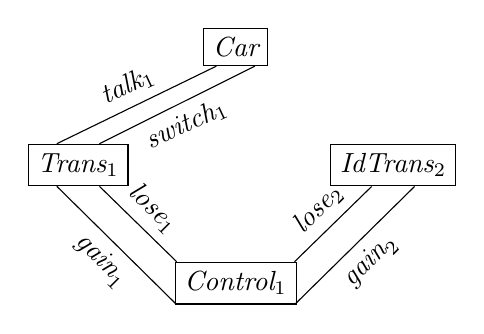
\begin{tikzpicture}
                \node[draw] (car) at (0, 0) {$\textit{Car}$};
                \node[draw] (trans) at (-2, -1.5) {$\textit{Trans}_1$};
                \node[draw] (idtrans) at (2, -1.5) {$\textit{IdTrans}_2$};
                \node[draw] (control) at (0, -3) {$\textit{Control}_1$};

                \draw (car.-135) -- node[above, rotate=25] {$\textit{talk}_1$}  (trans.135);
                \draw (car.-45) -- node[below, rotate=25] {$\textit{switch}_1$}  (trans.45);

                \draw (trans.-135) -- node[below, rotate=-45] {$\textit{gain}_1$} (control.-160);
                \draw (trans.-45) -- node[above, rotate=-45] {$\textit{lose}_1$} (control.160);

                \draw (idtrans.-135) -- node[above, rotate=45] {$\textit{lose}_2$} (control.20);
                \draw (idtrans.-45) -- node[below, rotate=45] {$\textit{gain}_2$} (control.-20);
            \end{tikzpicture}
        \end{subfigure}
        \hfill
        \begin{subfigure}{0.45\textwidth}
            \centering
            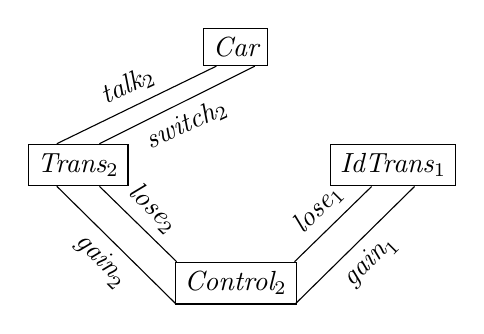
\begin{tikzpicture}
                \node[draw] (car) at (0, 0) {$\textit{Car}$};
                \node[draw] (trans) at (-2, -1.5) {$\textit{Trans}_2$};
                \node[draw] (idtrans) at (2, -1.5) {$\textit{IdTrans}_1$};
                \node[draw] (control) at (0, -3) {$\textit{Control}_2$};

                \draw (car.-135) -- node[above, rotate=25] {$\textit{talk}_2$}  (trans.135);
                \draw (car.-45) -- node[below, rotate=25] {$\textit{switch}_2$}  (trans.45);

                \draw (trans.-135) -- node[below, rotate=-45] {$\textit{gain}_2$} (control.-160);
                \draw (trans.-45) -- node[above, rotate=-45] {$\textit{lose}_2$} (control.160);

                \draw (idtrans.-135) -- node[above, rotate=45] {$\textit{lose}_1$} (control.20);
                \draw (idtrans.-45) -- node[below, rotate=45] {$\textit{gain}_1$} (control.-20);
            \end{tikzpicture}
        \end{subfigure}
    \end{figure}

    We will use parametrised recursive program definitions instead of replication and send/receive with multiple messages. We will later see how to translate recursive definitions into replication. 
    
    \textit{Trans} is parametrised by the channels it shares with \textit{Control}, which are \textit{lose} and \textit{gain}. On the other hand, \textit{Car} is parametrised by \textit{talk} and \textit{switch}. It can either \textit{talk} or obey an instruction to \textit{lose} the connection.

    \textit{IdTrans} is the idle transmitter. It is parametrised by the channels it shares with \textit{Control}, i.e. \textit{lose} and \textit{gain}. It can obey an instruction to gain a connection.

    Putting this all together, we get:
    \begin{align*}
        \textit{Trans}(\textit{talk}, \textit{switch}, \textit{gain}, \textit{lose}) &= \textit{talk}().\textit{Trans}(\textit{talk}, \textit{switch}, \textit{gain}, \textit{lose}) \\
        &+ \textit{lose}(t, s).\overline{\textit{switch}}\langle t, s \rangle.\textit{IdTrans}(\textit{gain}, \textit{lose}) \\
        \textit{IdTrans}(\textit{gain}, \textit{lose}) &= \textit{gain}(t, s).\textit{Trans}(t, s, \textit{gain}, \textit{lose})
    \end{align*}
    \noindent Note that the process $\textit{talk}()$ receives no messages- its mere purpose is synchronisation.

    \textit{Control} will either be $\textit{Control}_1$ or $\textit{Control}_2$. \textit{Control} can tell one transmitter to lose a connection and the other to gain a connection. We ignore how it decides this. So, we have:
    \begin{align*}
        \textit{Control}_1 &= \overline{\textit{lose}_1} \langle \textit{talk}_2, \textit{switch}_2 \rangle.\overline{\textit{gain}_2} \langle \textit{talk}_2, \textit{switch}_2 \rangle.\textit{Control}_2 \\
        \textit{Control}_2 &= \overline{\textit{lose}_2} \langle \textit{talk}_1, \textit{switch}_1 \rangle.\overline{\textit{gain}_1} \langle \textit{talk}_1, \textit{switch}_1 \rangle.\textit{Control}_1
    \end{align*}
    When we put everything together, the $\textit{lose}_i$, $\textit{talk}_i$ and $\textit{switch}_i$ channels will be in scope for $i \in \{1, 2\}$.

    Now, the \textit{Car} can either \textit{talk} or \textit{switch} to a new pair of channels. We would expect \textit{switch} to have priority over \textit{talk}, but this is not enforced. The definition of \textit{Car} is therefore the following:
    \[\textit{Car}(\textit{talk}, \textit{switch}) = \overline{\textit{talk}}\langle \rangle.\textit{Car} (\textit{talk}, \textit{switch}) + \textit{switch} (t, s).\textit{Car}(t, s)\]

    Finally, we define $\textit{System}_1$, with the starting state $\textit{Trans}_1$. This is given by:
    \begin{align*}
        \textit{System}_1 &= (\nu \ \textit{talk}_1, \textit{switch}_1, \textit{gain}_1, \textit{lose}_1, \textit{talk}_2, \textit{switch}_2, \textit{gain}_2, \textit{lose}_2) \\
        &\qquad (\textit{Car}(\textit{talk}_1, \textit{switch}_1) \mid \textit{Trans}_1 \mid \textit{IdTrans}_2 \mid \textit{Control}_1)
    \end{align*}
    where for $i \in \{1, 2\}$,
    \begin{align*}
        \textit{Trans}_i &= \textit{Trans}(\textit{talk}_i, \textit{switch}_i, \textit{gain}_i, \textit{lose}_i) \\
        \textit{IdTrans}_i &= \textit{IdTrans}(\textit{gain}_i, \textit{lose}_i) 
    \end{align*}
    We can define $\textit{System}_2$ in an analogous manner.

    Using this definition, we can reduce $\textit{System}_1$ reduces to $\textit{System}_2$:
    \begin{align*}
        \textit{Car}(\textit{talk}_1, \textit{switch}_1) &\mid \textit{Trans}_1 \mid \textit{IdTrans}_2 \mid \textit{Control}_1 \\
        &\equiv \\
        \textit{Car}(\textit{talk}_1, \textit{switch}_1) &\mid \dots + \textit{lose}(t, s).\dots \mid \textit{IdTrans}_2 \mid \overline{\textit{lose}_1} \langle \textit{talk}_2, \textit{switch}_2 \rangle \dots \\
        &\downarrow \\
        \dots + \textit{switch}(t, s).\dots &\mid \overline{\textit{switch}} \langle \textit{talk}_2, \textit{switch}_2 \rangle.\dots \mid \textit{IdTrans}_2 \mid \overline{\textit{gain}_2} \dots \\
        &\downarrow \\
        \textit{Car}(\textit{talk}_2, \textit{switch}_2) &\mid \textit{IdTrans}_1 \mid \textit{gain}_2(t, s)\dots \mid \overline{\textit{gain}_2} \langle \textit{talk}_2, \textit{switch}_2 \rangle \dots \\
        &\downarrow \\
        \textit{Car}(\textit{talk}_2, \textit{switch}_2) &\mid \textit{IdTrans}_1 \mid \textit{Trans}_2 \mid \textit{Control}_2
    \end{align*}

    % TODO: Modify the definition so that the new \textit{switch} and \textit{talk} channels are created every time the active \textit{Trans} changes.

    We defined \textit{Car} as follows:
    \[\textit{Car}(\textit{talk}, \textit{switch}) = \overline{\textit{talk}} \langle \rangle.\textit{Car} (\textit{talk}, \textit{switch}) + \textit{switch} (t, s).\textit{Car}(t, s)\]
    This is recursive parametrised definition of \textit{Car}. We can write it using replication using a replicated process that receives \textit{talk} and \textit{switch} on a channel called \textit{start}. We first define \textit{NewCar}:
    \[\textit{NewCar} = !(\textit{start}(t, s).(
        \overline{\textit{talk}} \langle \rangle.\overline{\textit{start}}\langle t, s \rangle.0 + 
        \textit{switch}(x, y).\overline{start} \langle x, y \rangle.0
    ))\]
    We can now replace $\textit{Car}(\textit{talk}_1, \textit{switch}_1)$ with:
    \[(\nu \ \textit{start})(\overline{\textit{start}} \langle \textit{talk}_1, \textit{switch}_1 \rangle.0 \mid \textit{NewCar})\]

    That way, we can reduce the following process:
    \begin{align*}
        \overline{\textit{start}} \langle \textit{talk}_1, \textit{switch}_1 \rangle.0 &\mid \textit{NewCar} \mid \textit{talk}_1().0 \\
        &\downarrow \\
        \overline{\textit{start}} \langle \textit{talk}_1, \textit{switch}_1 \rangle.0 \mid \textit{start}(t, s)\dots &\mid \textit{NewCar} \mid \textit{talk}_1().0 \\
        &\downarrow \\
        0 \mid \overline{\textit{talk}} \langle \rangle \dots + \dots &\mid \textit{NewCar} \mid \textit{talk}_1().0 \\
        &\downarrow \\
        0 \mid \overline{\textit{start}} \langle \textit{talk}_1, \textit{switch}_1 \rangle.0 &\mid \textit{NewCar} \mid 0 \\
        &\equiv \\
        \overline{\textit{start}} \langle \textit{talk}_1, \textit{switch}_1 \rangle.0 &\mid \textit{NewCar}
    \end{align*}
    During the process, we were able to \textit{talk} to the car.

    \subsection{Computation in $\pi$-calculus}
    In this section, we discuss how we can represent booleans and natural numbers in $\pi$-calculus.

    In $\pi$-calculus, we can represent a boolean value by a process that is given two channels and communicates on one of them. This is similar to the $\lambda$-calculus representation, but we now also need to specify a channel for interaction with the boolean; this is called its \emph{location}. We have
    \[\textit{True}(a) = a(t, f).\overline{t}\langle\rangle.0 \qquad \textit{False}(a) = a(t, f).\overline{f}\langle\rangle.0\]
    We can abbreviate definitions by omitting the $0$ at the end and empty braces. For instance, we have
    \[\textit{True}(a) = a(t, f).\overline{t}\]

    We can define a choice between processes $P$ and $Q$ on a boolean located at channel $a$. This is given by:
    \[\textit{Cond}(P, Q)(a) = (\nu \ t, f)\overline{a} \langle t, f \rangle.(t.P + f.Q)\]
    We illustrate how this works with an example. In particular, consider the following reduction:
    \begin{align*}
        \textit{True}(a) &\mid \textit{Cond}(P, Q)(a) \\
        &\equiv \\
        (\nu \ t, f) (a(t, f).\overline{t} &\mid \overline{a} \langle t, f \rangle.(t.P + f.Q)) \\
        &\downarrow \\
        (\nu \ t, f) (\overline{t} &\mid t.P + f.Q) \\
        &\downarrow \\
        (\nu \ t, f) (0 &\mid P) \\
        &\equiv \\
        &P
    \end{align*}

    Similarly,
    \[\textit{False}(a) \mid \textit{Cond}(P, Q)(a) \to^* Q\]

    Next, we can define the process $\textit{Not}(a, b)$, where $b$ is where the boolean currently is located, and $a$ is where it will be after the negation process. This process is given by:
    \[\textit{Not}(a, b) = (\nu \ t, f)(\overline{b} \langle t, f \rangle.(
        t.\textit{False}(a) + f.\textit{True}(a)
    ))\]
    We illustrate this with the following reduction:
    \begin{align*}
        \textit{Not}(a, b) &\mid \textit{True}(b) \\
        &\equiv \\
        (\nu \ t, f)(\overline{b} \langle t, f \rangle.(t.\textit{False}(a) + f.\textit{True}(a)) &\mid b(t, f).\overline{t}) \\
        &\downarrow \\
        (\nu \ t, f)(t.\textit{False}(a) + f.\textit{True}(a) &\mid \overline{t} ) \\
        &\downarrow \\
        (\nu \ t, f)(\textit{False}(a) &\mid 0) \\
        &\equiv \\
        \textit{False}(a)
    \end{align*}

    We now define the process $\textit{And}(a, b, c)$, which takes in two booleans at $b$ and $c$ and produces a boolean at $a$. This is given by:
    \[\textit{And}(a, b, c) = (\nu t, f)(\overline{b} \langle t, f \rangle.(
        f.\textit{False}(a) + t.\overline{c} \langle t, f \rangle.(
            f.\textit{False}(a) + t.\textit{True}(a)
        )
    ))\]
    We can reduce to find that
    \begin{align*}
        \textit{And}(a, b, c) \mid \textit{True}(b) \mid \textit{True}(c) &\to^* \textit{True}(a) \\
        \textit{And}(a, b, c) \mid \textit{True}(b) \mid \textit{False}(c) &\to^* \textit{False}(a)
    \end{align*}

    We will now use a similar idea to represent natural numbers. It is more direct than in $\lambda$-calculus since we do not need \texttt{pair}. We define it recursively, with
    \begin{align*}
        Z(n_0) &= n_0(z, s).\overline{z} \\
        S(n_k, N(n_{k-1})) &= (\nu \ n_{k-1})(n_k(z, s).\overline{s} \langle n_{k-1} \rangle \mid N(n_{k-1}))
    \end{align*}
    This way, we represent the value $\textit{One}$ as follows:
    \[\textit{One}(n_1) \equiv S(n_1, Z(n_0)) \equiv (\nu \ n_1)(n_1(z, s) \overline{s} \langle n_0 \rangle \mid n_0(z, s).\overline{z})\]
    
    Like \textit{Cond} for booleans, we can define a case-analysis process for natural numbers, as follows:
    \[\textit{Cases}(P, Q)(a, n) = (\nu \ z, s)\overline{a} \langle z, s \rangle.(z.P + s(n).Q(n)).\]
    The process \textit{Cases} interacts with a number located at $a$. If it is zero, it will next perform $P$; if it is instead the successor of $n$, then it will continue as $Q(n)$. Using this, we can define the \textit{IsZero} process:
    \[\textit{IsZero}(a, n) = \textit{Cases}(\textit{True}(a), \textit{False}(a))(n, m).\]
    We illustrate how the process works with two examples, first running it in parallel with zero:
    \begin{align*}
        \textit{IsZero}(a, n_0) &\mid Z(n_0) \\
        &\equiv \\
        \textit{Cases}(\textit{True}(a), \textit{False}(a))(n_0, m) &\mid n_0(z, s).\overline{z} \\
        &\equiv \\
        (\nu \ z, s)(\overline{n_0} \langle z, s \rangle.(z.\textit{True}(a) + s(m).\textit{False}(a)) &\mid n_0(z, s).\overline{z}) \\
        &\downarrow \\
        (\nu \ z, s)(z.\textit{True}(a) + s(m).\textit{False}(a) &\mid \overline{z}) \\
        &\downarrow \\
        (\nu \ z, s)(\textit{True}(a) &\mid 0) \\
        &\equiv \\
        \textit{True}(a)
    \end{align*}
    Now, we run \textit{isZero} in parallel with \textit{One}:
    \begin{align*}
        \textit{IsZero}(a, n_1) &\mid \textit{One}(n_1) \\
        &\equiv \\
        (\nu \ z, s, n_1)(\overline{n_1} \langle z, s \rangle.(z.\textit{True}(a) + s(m).\textit{False}(a)) &\mid n_1(z, s). \overline{s} \langle n_0 \rangle \mid n_0(z, s).\overline{z}) \\
        &\downarrow \\
        (\nu \ z, s, n_1)(z.\textit{True}(a) + s(m).\textit{False}(a) &\mid \overline{s} \langle n_0 \rangle \mid n_0(z, s).\overline{z}) \\
        &\downarrow \\
        (\nu \ z, s, n_1)(\textit{False}(a) &\mid 0 \mid n_0(z, s).\overline{z}) \\
        &\equiv \\
        \textit{False}(a) &\mid n_0(z, s).\overline{z}
    \end{align*}
    We have gotten the \textit{False} result, and the two remaining processes cannot interact.

    We will now define the \textit{even} process in $\pi$-calculus. Formally, the \textit{even} function can be defined as follows:
    \begin{align*}
        \textit{even}(Z) &= \textit{true} \\
        \textit{even}(S(n)) &= \textit{not}(\textit{even}(n))
    \end{align*}
    In $\pi$-calculus, we can define \textit{Even} using replication. This is given as follows:
    \begin{align*}
        \textit{Even} &= !(\textit{even}(a, n).\textit{Cases}(\textit{True}(a), 
            (\nu \ b)(\textit{Not}(a, b) \mid \overline{\textit{even}} \langle b, m \rangle)(n, m)
        ))
    \end{align*}
    The channel where we check is \textit{even}. The value that we are checking is $n$, and the result is outputted into channel $a$. We run the process on some number $N$ at $n_k$ using the process
    \[(\nu \ n_k)(\overline{\textit{even}}\langle a, n_k\rangle \mid N(n_k) \mid \textit{Even})\]
    For instance, we can run it on the zero process as follows:
    \begin{align*}
        \overline{\textit{even}} \langle a, n_0\rangle \mid Z(n_0) &\mid \textit{Even} \\
        &\equiv \\
        \overline{\textit{even}} \langle a, n_0\rangle \mid n_0(z, s).\overline{z} \mid \textit{even}(a, n_0)\dots &\mid \textit{Even} \\
        &\downarrow \\
        (\nu \ z, s) (0 \mid n_0\langle z, s \rangle.\overline{z} \mid \overline{n_0}\langle z, s \rangle\dots) &\mid \textit{Even} \\
        &\downarrow \\
        (\nu \ z, s)(z \mid z.\textit{True}(a) + \dots) &\mid \textit{Even} \\
        &\downarrow \\
        (\nu \ z, s)(0 \mid \textit{True}(a)) &\mid \textit{Even} \\
        &\equiv \\
        \textit{True}(a) &\mid \textit{Even}
    \end{align*}
    Next, we run it on the \textit{One} process:
    \begin{align*}
        \overline{\textit{even}} \langle a, n_1 \rangle \mid \textit{One}(n_1) &\mid \textit{Even} \\
        &\equiv \\
        (\nu \ n_1)(\overline{\textit{even}} \langle a, n_1\rangle \mid n_1(z, s).\overline{s} \langle n_0 \rangle \mid n_0(z, s).\overline{z} \mid \textit{even}(a, n_1)\dots) &\mid \textit{Even} \\
        &\downarrow \\
        (\nu \ z, s, n_1)(0 \mid n_1(z, s).\overline{s} \langle n_0 \rangle \mid n_0(z, s).\overline{z} \mid n_1\langle z, s \rangle \dots) &\mid \textit{Even} \\
        &\downarrow \\
        (\nu \ b, z, s, n_1)(\overline{s} \langle n_0 \rangle \mid n_0(z, s).\overline{z} \mid \dots + s(m).(\textit{Not}(a, b) \mid \overline{\textit{even}}(b, m))) &\mid \textit{Even} \\
        &\downarrow \\
        (\nu \ z, s, n_1)(0 \mid n_0(z, s).\overline{z} \mid \textit{Not}(a, b) \mid \overline{\textit{even}}(b, n_0)) &\mid \textit{Even} \\
        &\equiv \\
        (\nu \ b)(\textit{Not}(a, b) \mid \overline{\textit{even}} \langle b, n_0\rangle \mid Z(n_0)) &\mid \textit{Even} \\
        &\downarrow_* \\
        (\nu \ b)(\textit{Not}(a, b) \mid \textit{True}(b)) &\mid \textit{Even} \\
        &\downarrow_* \\
        \textit{False}(a) &\mid \textit{Even}
    \end{align*}

    The example of the even function looks complicated because it combined two ideas:
    \begin{itemize}
        \item the encoding of natural numbers as processes; and
        \item the use of replication to express a recursive function definition.
    \end{itemize}
    We can explain the second point more easily if we assume that we extend $\pi$-calculus with integers, booleans, expressions formed from standard operations, reduction of boolean and integer expressions, and a condition construct
    \[\textit{if } e \textit{ then } P \textit{ else } Q.\]
    It has the following reduction rules:
    \[\textit{if } \texttt{true} \textit{ then } P \textit{ else } Q \to P \qquad \textit{if } \texttt{false} \textit{ then } P \textit{ else } Q \to Q \]
    \[\frac{e \to e'}{\textit{if } e \textit{ then } P \textit{ else } Q \to \textit{if } e' \textit{ then } P \textit{ else } Q}\]
    That way, we can write the \textit{even} process as follows:
    \[\textit{Even} = !(
        \textit{even}(n).(\textit{if IsZero}(n)\textit{ then }\texttt{true} \textit{ else not(Even(n-1))})
    )\]
    We can write the factorial function in a similar manner:
    \[\textit{Fact} = !(
        \textit{fact}(a, n).\textit{if isZero}(n)\textit{ then }\overline{a} \langle 1 \rangle 
        \textit{ else }(\nu \ b)(\overline{\textit{fact}} \langle b, n-1 \rangle \mid b(x).\overline{a} \langle n \cdot x \rangle)
    )\]
    % TODO: Check that fact(a, 1) = \overline{a} \langle 1 \rangle \mid Fact

    Note that the functions defined above consume the number they interact with. This makes it impossible to define functions that use their arguments more than once. It is possible to define persistent versions of the booleans and natural numbers, by using replication, e.g. $\textit{True}(a) = !(a(t, f).\overline{t})$.

    Using these examples, and a formal proof, we can see that $\pi$-calculus can express all computable functions. It is possible to prove this by defining a translation from $\lambda$-calculus into $\pi$-calculus, or by directly showing that all recursive functions on natural numbers can be defined in $\pi$-calculus.

    There is an argument that $\pi$-calculus is more fundamental than $\lambda$-calculus because $\pi$-calculus can easily express functional behaviour in terms of communication, whereas modeling concurrency behaviour in $\lambda$-calculus would require elaborate encodings.
    \newpage

    \section{Equivalence of Process}
    Part of the motivation for the topic of process calculus is to be able to reason about \emph{communicating concurrent systems}: to specify how they behave and verify that they behave correctly.

    The first step was to define the syntax and operational semantics, i.e. the reduction relation. We have also seen how to define some interesting computational scenarios involving concurrency and communication.

    We will now introduce a \emph{theory of equivalence of processes}, which means equivalence of ongoing interactive behaviour. This is in contrast with $\lambda$-calculus, where we had an equivalence of the final result.

    Previously, we define the processes $\textit{True}(x)$ and $\textit{False}(x)$, and $\textit{Not}(x, y)$. We would like to have a theory in which
    \[(\nu \ y)(\textit{Not}(x, y) \mid \textit{True}(y)) = \textit{False}(x).\]
    The fact that $\textit{False}(x)$ represents the boolean value \textit{false} is to do with the way it interacts on the channel $x$, so the definition of equivalent must take that into account. Moreover, applying \textit{Not} twice should be the identity function on booleans, i.e.
    \[x(t, f).\overline{y} \langle t, f \rangle = (\nu \ z)(\textit{Not}(x, z) \mid \textit{Not}(z, y))\]

    To develop the theory of equivalence, we will simplify $\pi$-calculus by assuming that all messages are empty. To reduce syntax, we will omit the empty messages and just write $x$ or $\overline{x}$. We will refer to $x$ and $\overline{x}$ as actions. This means that we are working in an earlier process calculus called CCS-calculus of Communication Systems. We will start with examples and then give proper definitions.

    \subsection{Trace Equivalence}
    Reductions of the form $P \to Q$ tell us how a process evolves by \emph{internal} communication. We need to be able to describe \emph{potential} interaction between a process and its environment. We do this by introducing \emph{labelled} transitions, e.g.
    \[a.P \xrightarrow{a} P \qquad \overline{a}.Q \xrightarrow{\overline{a}} Q\]
    We can describe actual interactions using $\tau$ transitions, e.g.
    \[a.P \mid \overline{a}.Q \xrightarrow{\tau} P \mid Q\]

    We will now define labelled transitions. Let $\alpha \in \{a, \overline{a}, \tau\}$. Then, the inference rules for labelled transitions are given as follows:
    \[\overline{\alpha.P \xrightarrow{\alpha} P}\]
    \[\frac{P \xrightarrow{a} P' \quad Q \xrightarrow{\overline{a}} Q'}{P \mid Q \xrightarrow{\tau} P' \mid Q'} \qquad \frac{P \xrightarrow{\overline{a}} P' \quad Q \xrightarrow{a} Q'}{P \mid Q \xrightarrow{\tau} P' \mid Q'}\]
    \[\frac{P \xrightarrow{\alpha} P'}{P \mid Q \xrightarrow{\alpha} P' \mid Q} \qquad \frac{Q \xrightarrow{\alpha} Q'}{P \mid Q \xrightarrow{\alpha} P \mid Q'}\]
    \[\frac{P \xrightarrow{\alpha} P'}{P + Q \xrightarrow{\alpha} P' + Q} \qquad \frac{Q \xrightarrow{\alpha} Q'}{P + Q \xrightarrow{\alpha} P + Q'}\]
    \[\frac{P \xrightarrow{\alpha} P' \quad \alpha \not\in \{y, \overline{y}\}}{(\nu \ y)P \xrightarrow{\alpha} (\nu \ y)P'}\]
    \[\frac{P \xrightarrow{\alpha} P'}{!P \xrightarrow{\alpha} P' \mid !P} \qquad \frac{P \xrightarrow{\overline{a}} P' \quad P \xrightarrow{a} P''}{!P \xrightarrow{\tau} (P' \mid P'') \mid !P}\]

    We can now talk about \emph{traces} of a process, which are its possible sequences of actions. The empty trace $\epsilon$ is always a possibility. We look at some examples:
    \begin{itemize}
        \item $a.b.0$ has traces $\epsilon$, $a$, $ab$;
        \item $a.0 + b.0$ has traces $\epsilon$, $a$, $b$;
        \item $a.\overline{b}.0 + b.0$ has traces $\epsilon$, $a$, $b$, $a\overline{b}$; and
        \item $a.b.0 + b.\overline{c}.0 + \overline{c}.0$ has traces $\epsilon$, $a$, $b$, $\overline{c}$, $ab$, $b\overline{c}$.
    \end{itemize}

    We can show the labelled transitions of a process in a diagram, with or without the process terms. We can then read off the traces. For example, the process $a.\overline{b}.0 + b.0$ corresponds to the following figure:
    \begin{figure}[H]
        \centering
        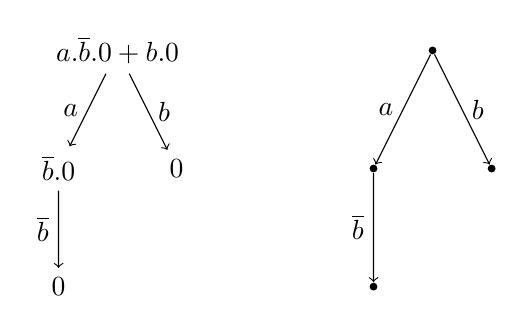
\begin{tikzpicture}
            \node at (0, 0) {$a.\overline{b}.0 + b.0$}
            child {
                node {$\overline{b}.0$}
                child {
                    node {$0$}
                    edge from parent[->] node[left] {$\overline{b}$}
                }
                edge from parent[->] node[left] {$a$}
            }
            child {
                node {$0$}
                edge from parent[->] node[right] {$b$}
            };

            \node[circle, fill, inner sep=1pt] at (4, 0) {}
            child {
                node[circle, fill, inner sep=1pt] {}
                child {
                    node[circle, fill, inner sep=1pt] {}
                    edge from parent[->] node[left] {$\overline{b}$}
                }
                edge from parent[->] node[left] {$a$}
            }
            child {
                node[circle, fill, inner sep=1pt] {}
                edge from parent[->] node[right] {$b$}
            };
        \end{tikzpicture}
    \end{figure}
    \noindent On the left, we highlight all the processes, while on the right, we only show the traces.

    A simple equivalence between processes is \emph{trace equivalence}. We say that $P =_{tr} Q$ if they have the same traces. For example, $(\nu \ b)(a.\overline{b}.0 \mid b.c.0)$ and $a.\tau.c.0$ are trace equivalent since they have the same traces:
    \begin{figure}[H]
        \centering
        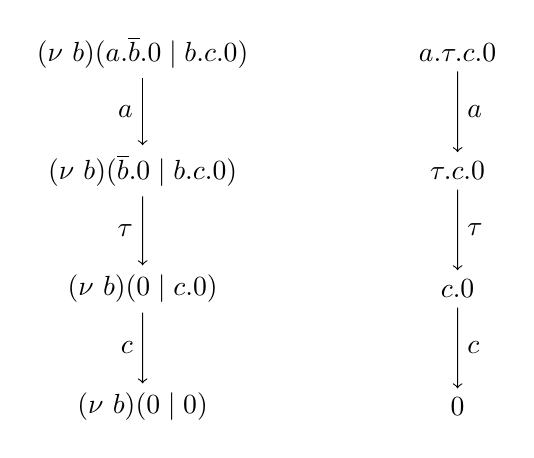
\begin{tikzpicture}
            \node at (0, 0) {$(\nu \ b)(a.\overline{b}.0 \mid b.c.0)$}
            child {
                node {$(\nu \ b)(\overline{b}.0 \mid b.c.0)$}
                child {
                    node {$(\nu \ b)(0 \mid c.0)$}
                    child {
                        node {$(\nu \ b)(0 \mid 0)$}
                        edge from parent[->] node[left] {$c$}
                    }
                    edge from parent[->] node[left] {$\tau$}
                }
                edge from parent[->] node[left] {$a$}
            };
            
            \node at (4, 0) {$a.\tau.c.0$}
            child {
                node {$\tau.c.0$}
                child {
                    node {$c.0$}
                    child {
                        node {$0$}
                        edge from parent[->] node[right] {$c$}
                    }
                    edge from parent[->] node[right] {$\tau$}
                }
                edge from parent[->] node[right] {$a$}
            };
        \end{tikzpicture}
    \end{figure}
    \noindent Since the channel $b$ is private, note that $(\nu \ b)(a.\overline{b}.0 \mid b.c.0)$ cannot have a $b$-trace.

    \subsection{Informal introduction to bisimulation}
    There is an issue with trace equivalence- it is too weak. To see this, consider the two processes $P = a.b.0 + a.c.0$ and $Q = a.(b.0 + c.0)$. They have the following trace diagrams:
    \begin{figure}[H]
        \centering
        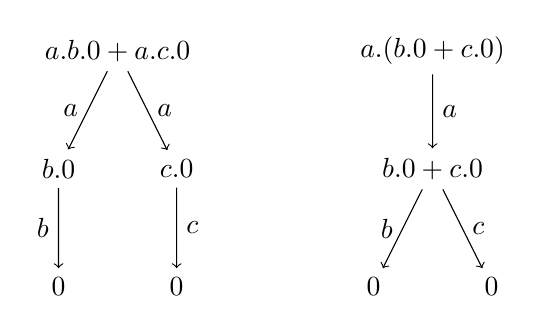
\begin{tikzpicture}
            \node at (0, 0) {$a.b.0 + a.c.0$}
            child {
                node {$b.0$}
                child {
                    node {$0$}
                    edge from parent[->] node[left] {$b$}
                }
                edge from parent[->] node[left] {$a$}
            }
            child {
                node {$c.0$}
                child {
                    node {$0$}
                    edge from parent[->] node[right] {$c$}
                }
                edge from parent[->] node[right] {$a$}
            };

            \node at (4, 0) {$a.(b.0 + c.0)$}
            child {
                node {$b.0 + c.0$}
                child {
                    node{$0$}
                    edge from parent[->] node[left] {$b$}
                }
                child {
                    node{$0$}
                    edge from parent[->] node[right] {$c$}
                }
                edge from parent[->] node[right] {$a$}
            };
        \end{tikzpicture}
    \end{figure}
    \noindent Both the processes have traces $\epsilon$, $a$, $ab$ and $ac$. Hence, they are trace equivalent. However, after an $a$-reduction, $P$ can go into a state in which only one of $b$ and $c$ is available, whereas $Q$ offers both $b$ and $c$. 

    We illustrate the issue further. Define $R = \overline{a}.\overline{b}.0$. If we have the process $Q \mid R$, then we can reduce it as follows:
    \begin{align*}
        a.(b.0 + c.0) &\mid \overline{a}.\overline{b}.0 \\
        &\downarrow \\
        b.0 + c.0 &\mid \overline{b}.0 \\
        &\downarrow \\
        0 &\mid 0
    \end{align*}
    This is the only reduction possible from $Q \mid R$. So, every reduction leads to termination in this case. On the other hand, if we have the process $P \mid R$, it could reduce in two ways:
    \begin{align*}
        a.b.0 + a.c.0 &\mid \overline{a}.\overline{b}.0  & a.b.0 + a.c.0 &\mid \overline{a}.\overline{b}.0 \\
        &\downarrow & &\downarrow \\
        c.0 &\mid \overline{b}.0 & b.0 &\mid \overline{b}.0 \\
        & & &\downarrow \\
        & & 0 &\mid 0
    \end{align*}
    Since $\overline{a}.\overline{b}.0$ can communicate with $a.c.0$ at the top level, there is nothing stopping the left reduction from happening. However, this reduction leads to a deadlock. On the other hand, no reduction of $Q \mid R$ leads to a deadlock. We would like the equivalence of process to be deadlock-invariant, i.e. if two processes are equivalent, then either they both can reduce to a deadlock or neither can.

    To do this, we define \emph{bisimulation}. This concept is fundamental in process calculus and concurrency theory.

    There are many forms of bisimulation. We look at \emph{strong bisimulation}. The idea is that for processes $P$ and $Q$ to be bisimilar, it must be that:
    \begin{itemize}
        \item for any action $\alpha \in \{a, \overline{a}, \tau\}$, if $P \xrightarrow{\alpha} P'$, then there is a $Q'$ such that $Q \xrightarrow{\alpha} Q'$ and $P'$ and $Q'$ are bisimilar;
        \item this holds the other way as well, i.e. when $Q \xrightarrow{\alpha} Q'$, then there exists a $P'$ bisimilar to $Q'$ such that $P \xrightarrow{\alpha} P'$ as well.
    \end{itemize}

    We now consider the processes $P = (\nu \ b)(a.\overline{b}.0 \mid b.c.0)$ and $Q = a.\tau.c.0$. We previously saw that the two processes were trace equivalent. We will now see that they are also bisimilar, since they have the same trace diagram:
    \begin{figure}[H]
        \centering
        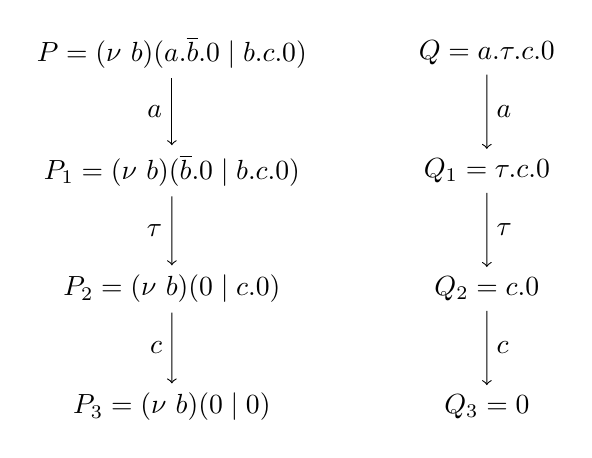
\begin{tikzpicture}
            \node at (0, 0) {$P = (\nu \ b)(a.\overline{b}.0 \mid b.c.0)$}
            child {
                node {$P_1 = (\nu \ b)(\overline{b}.0 \mid b.c.0)$}
                child {
                    node {$P_2 = (\nu \ b)(0 \mid c.0)$}
                    child {
                        node {$P_3 = (\nu \ b)(0 \mid 0)$}
                        edge from parent[->] node[left] {$c$}
                    }
                    edge from parent[->] node[left] {$\tau$}
                }
                edge from parent[->] node[left] {$a$}
            };
            
            \node at (4, 0) {$Q = a.\tau.c.0$}
            child {
                node {$Q_1 = \tau.c.0$}
                child {
                    node {$Q_2 = c.0$}
                    child {
                        node {$Q_3 = 0$}
                        edge from parent[->] node[right] {$c$}
                    }
                    edge from parent[->] node[right] {$\tau$}
                }
                edge from parent[->] node[right] {$a$}
            };
        \end{tikzpicture}
    \end{figure}

    We can work from the end to prove that $P$ and $Q$ are bisimilar. We use the symbol $\sim$ for strong bisimulation. In this case, $P_3 \sim Q_3$ because neither of them has any transitions; they are both structurally congruent to $0$. So, there is nothing to check here. Now, consider $P_2$ and $Q_2$. We have $P_2 \xrightarrow{c} P_3$, which can be matched by $Q_2 \xrightarrow{c} Q_3$, and we know that $P_3 \sim Q_3$. In the other direction, the only transition of $Q_2$ is $Q_2 \xrightarrow{c} Q_3$, which can equally be matched by $P_2 \xrightarrow{c} P_3$, with $P_3 \sim Q_3$.

    Similarly, we can show that $P_1 \sim Q_1$- the only transition of $P_1$ is $P_1 \xrightarrow{\tau} P_2$ from communication on $b$. This can be matched by $Q_1 \xrightarrow{\tau} Q_2$, and we know that $P_2 \sim Q_2$. In the other direction, the only transition of $Q_1$ is $Q_1 \xrightarrow{\tau} Q_2$, which can be matched by $P_1 \xrightarrow{\tau} P_2$, and we know that $P_2 \sim Q_2$. 

    Finally, we consider the transitions of $P$ and $Q$ in the same way. We can see that each process has an $a$-transition that can match the $a$-transition of the other process, resulting in $P_1$ and $Q_1$, with $P_1 \sim Q_1$. We conclude that $P \sim Q$. Note that $b$ is a private channel in $P_1$, meaning that $P_1$ cannot fire a $b$-transition.

    Now, consider $P = a.b.0 + a.c.0$ and $Q = a.(b.0 + c.0)$. We saw that $P$ and $Q$ were trace equivalent. However, they are not bisimilar- consider the trace diagram for $P$ and $Q$.
    \begin{figure}[H]
        \centering
        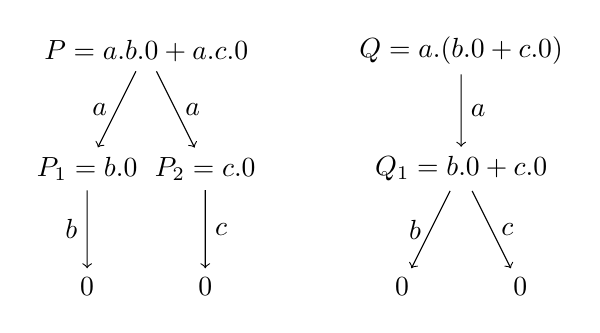
\begin{tikzpicture}
            \node at (0, 0) {$P = a.b.0 + a.c.0$}
            child {
                node {$P_1 = b.0$}
                child {
                    node {$0$}
                    edge from parent[->] node[left] {$b$}
                }
                edge from parent[->] node[left] {$a$}
            }
            child {
                node {$P_2 = c.0$}
                child {
                    node {$0$}
                    edge from parent[->] node[right] {$c$}
                }
                edge from parent[->] node[right] {$a$}
            };

            \node at (4, 0) {$Q = a.(b.0 + c.0)$}
            child {
                node {$Q_1 = b.0 + c.0$}
                child {
                    node{$0$}
                    edge from parent[->] node[left] {$b$}
                }
                child {
                    node{$0$}
                    edge from parent[->] node[right] {$c$}
                }
                edge from parent[->] node[right] {$a$}
            };
        \end{tikzpicture}
    \end{figure}
    \noindent We see that $P$ has two transitions- $P \xrightarrow{a} P_1$ and $P \xrightarrow{a} P_2$. We can match $P \xrightarrow{a} P_1$ by $Q \xrightarrow{a} Q_1$, so we would need $P_1 \sim Q_1$. Also, $P \xrightarrow{a} P_2$ is matched by $Q \xrightarrow{a} Q_1$. But, $Q_1$ has a transition $Q_1 \xrightarrow{b} 0$, which cannot be matched by $P_2$. So, we cannot have $P \sim Q$.

    We have found that strong bisimulation is a better definition of equivalence when we have non-determinism. This is because it takes into account how a process can interact with other processes. If two processes are strongly bisimilar, then they are also trace equivalent. If two deterministic processes are trace equivalent, then they are also strongly bisimilar.

    Note that the term `strong' means that we include $\tau$ transitions when matching. Sometimes, this is undesirable because $\tau$ transitions are supposed to be internal unobservable actions. There is another form of equivalence, \emph{weak bisimulation}, which ignores $\tau$ transitions.

    \subsection{Formal definition of bisimulation}
    We will now aim to define strong bisimulation. A first attempt might be the following:
    \begin{definition}
        We say that $P$ and $Q$ are \emph{strongly bisimilar}, denoted $P \sim Q$ if for every action $\alpha$:
        \begin{itemize}
            \item if $P \xrightarrow{\alpha} P'$, then there is a $Q'$ such that $Q \xrightarrow{\alpha} Q'$ and $P' \sim Q'$; and
            \item if $Q \xrightarrow{\alpha} Q'$, then there is a $P'$ such that $P \xrightarrow{\alpha} P'$ and $P' \sim Q'$.
        \end{itemize}
    \end{definition}
    This definition is recursive in nature. In the base case, the process will not have any action. However, there is no reason that $P'$ and $Q'$ get 'smaller' than $P$ and $Q$, so we might not be headed to the base case in general.

    We illustrate the issue further. So, consider the process $P = {!a.0}$. We would like $P \sim P$. Because $a.0 \xrightarrow{a} 0$, we have
    \[P \xrightarrow{a} 0 \mid {!a.0} \equiv 0 \mid P.\]
    Applying the above definition of strong bisimulation to $P$ both on the left and the right, we see that they can match each other's actions. Checking the subsequent processes tells us that $P \sim P$ depends on $0 \mid P \sim 0 \mid P$. This is circular and not a valid definition. Moreover, the reduced process is equivalent to itself, meaning that the reduced process does not get smaller.

    Instead of defining bisimulation for $\pi$-calculus processes, we can work with more abstract \emph{labelled transition systems} (LTS). An LTS is a directed graph in which edges are labelled with actions. We use the transition notation
    \[m \xrightarrow{a} n\]
    where $m$ and $n$ are nodes in the graph. We can think of an LTS as a transition diagram for processes, in which the nodes have $\pi$-calculus processes associated with them.

    The first step is to consider a general relation $\mathcal{R}$ on processes (or nodes of an LTS). If $P_1$ and $P_2$ are processes related by $\mathcal{R}$, we write $(P_1, P_2) \in \mathcal{R}$ or $P_1 \mathcal{R} P_2$. Now, we define the property of being a strong bisimulation, which is a property that a relation might or might not have.
    \begin{definition}
        A relation $\mathcal{R}$ on processes (or on nodes of an LTS) is a \emph{strong bisimulation} if whenever $P \mathcal{R} Q$, for every action $\alpha$, it is the case that
        \begin{itemize}
            \item if $P \xrightarrow{\alpha} P'$, then there is $Q'$ such that $Q \xrightarrow{\alpha} Q'$, and $P' \mathcal{R} Q'$; and
            \item if $Q \xrightarrow{\alpha} Q'$, then there is $P'$ such that $P \xrightarrow{\alpha} P'$, and $P' \mathcal{R} Q'$.
        \end{itemize}
    \end{definition}

    Consider the labelled transition system given below.
    \begin{figure}[H]
        \centering
        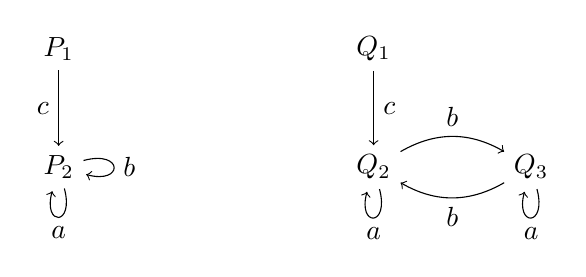
\begin{tikzpicture}
            \node (p1) at (0, 0) {$P_1$};
            \node (p2) at (0, -1.5) {$P_2$};

            \draw[->] (p1) edge node[left] {$c$} (p2);
            \draw[->] (p2) edge[loop below] node {$a$} (p2);
            \draw[->] (p2) edge[loop right] node {$b$} (p2);

            \node (q1) at (4, 0) {$Q_1$};
            \node (q2) at (4, -1.5) {$Q_2$};
            \node (q3) at (6, -1.5) {$Q_3$};

            \draw[->] (q1) edge node[right] {$c$} (q2);
            \draw[->] (q2) edge[bend left] node[above] {$b$} (q3);
            \draw[->] (q3) edge[bend left] node[below] {$b$} (q2);
            \draw[->] (q2) edge[loop below] node {$a$} (q2);
            \draw[->] (q3) edge[loop below] node {$a$} (q3);
        \end{tikzpicture}
    \end{figure}
    \noindent We consider which relations are bisimilar with respect to this LTS.
    \begin{itemize}
        \item The empty relation $\varnothing$ is a strong bisimulation- this is trivially the case.
        \item The relation $\{(P_2, Q_2)\}$ is not a strong bisimulation- we have $P_2 \xrightarrow{b} P_2$, but in $Q_2$, the only $b$-transition is to $Q_3$, but $(P_2, Q_3) \not\in \mathcal{R}$.
        \item The relation $\{(P_2, P_2)\}$ is a strong bisimulation since it can match all of its transitions.
        \item The relation $\{(P_2, Q_2), (P_2, Q_3)\}$ is a strong bisimulation- we have $P_2 \xrightarrow{b} P_2$ matching $Q_2 \xrightarrow{b} Q_3$ and $Q_3 \xrightarrow{b} Q_2$; and $P_2 \xrightarrow{a} P_2$ matching $Q_2 \xrightarrow{a} Q_2$ and $Q_3 \xrightarrow{a} Q_3$.
        \item The relation $\{(P_2, Q_2), (P_2, Q_3), (Q_2, P_2), (Q_3, P_2)\}$ is a strong bisimulation- we have added the symmetrical cases.
        \item The relation $\{(P_1, Q_1), (P_2, Q_2), (P_2, Q_3)\}$ is a strong bisimulation since $P_1 \xrightarrow{c} P_2$ is matched by $Q_1 \xrightarrow{c} Q_2$, with $(P_2, Q_2) \in \mathcal{R}$.
        \item The relation $\{(P_1, Q_1), (P_2, Q_2), (P_2, Q_3), (Q_1, P_1), (Q_2, P_2), (Q_3, P_2)\}$ is a strong bisimulation. Adding reflexivity (i.e. $(P, P)$ for all processes) to this relation would give us the largest possible set satisfying strong bisimulation.
    \end{itemize}

    For a given LTS (or a set of processes), there can be several relations that satisfy the conditions to be a strong bisimulation. We say that \emph{strong bisimilarity}, denoted by $\sim$, is the largest strong bisimulation. We say that processes $P$ and $Q$ are \emph{strongly bisimilar}, denoted $P \sim Q$, if $(P, Q)$ is in the largest strong bisimulation. To prove this, it is sufficient to find any bisimulation containing $(P, Q)$.

    Now, consider the following LTS:
    \begin{figure}[H]
        \centering
        \begin{tikzpicture}
            \node (p1) at (0, 0) {$P_1$};
            \node (p2) at (0, -1.5) {$P_2$};

            \draw[->] (p1) edge node[left] {$a$} (p2);
            \draw[->] (p2) edge[loop below] node {$a$} (p2);

            \node (q1) at (3, 0) {$Q_1$};
            \draw[->] (q1) edge[loop below] node {$a$} (q1);
        \end{tikzpicture}
    \end{figure}
    Then, the following are relations satisfying strong bisimulation:
    \begin{itemize}
        \item $\{(P_1, P_2), (P_2, P_2)\}$- we can match $P_1 \xrightarrow{a} P_2$ with $P_2 \xrightarrow{a} P_2$, and we have $(P_2, P_2) \in \mathcal{R}$, and vice versa;
        \item $\{(P_2, Q_1)\}$- we can match $P_2 \xrightarrow{a} P_2$ with $Q_1 \xrightarrow{a} Q_1$, with $(P_2, Q_1) \in \mathcal{R}$;
        \item $\{(P_1, Q_1), (P_2, Q_1)\}$- we can match $P_1 \xrightarrow{a} P_2$ with $Q_1 \xrightarrow{a} Q_1$, with $(P_2, Q_1) \in \mathcal{R}$.
    \end{itemize}
    By reflexivity and symmetry, the largest strong bisimulation is:
    \begin{align*}
        \{(P_1, P_1), (P_2, P_2), (Q_1, Q_1), (P_1, P_2), (P_2, P_1), \\
        (P_1, Q_1), (Q_1, P_1) (P_2, Q_1), (Q_2, P_1)\}.
    \end{align*}
    This implies that every process is strongly bisimilar in this case.

    We have previously used inductive definitions, e.g. the definitions of reduction and typing judgments. An inductive definition is when we define a set or relation to be the smallest entity satisfying certain conditions. Ordinary recursive function definitions are also in this category. A \emph{coninductive} definition is when we define a set or a relation to be the largest entity satisfying certain conditions, such as strong bisimilarity.

    We will now look at processes in the syntax $\pi$-calculus, rather than abstract LTS. When defining labelled transitions for $\pi$-calculus, we did not take structural congruence into account. So, if we want to show something like $P \mid Q$ and $Q \mid P$ to be bisimilar, we have to prove it by constructing a strong bisimulation that contains $(P \mid Q, Q \mid P)$. 
    
    \begin{proposition}
        Let $P$ and $Q$ be processes. Then $P \mid Q \sim Q \mid P$.
    \end{proposition}
    \begin{proof}
        To prove this, it suffices to show that there is a relation containing $(P \mid Q, Q \mid P)$. So, define the relation
        \[\mathcal{R} = \{(P \mid Q, Q \mid P) \mid P, Q \textrm{ processes}\}.\]
        We show that $\mathcal{R}$ is a strong bisimulation. So, let $(P \mid Q, Q \mid P) \in \mathcal{R}$ There are 3 transitions for $P \mid Q$:
        \begin{itemize}
            \item First assume that $P \mid Q \xrightarrow{\alpha} P' \mid Q$ because $P \xrightarrow{\alpha} P'$. In that case, we find that $Q \mid P \xrightarrow{\alpha} Q \mid P'$ by definition of parallel composition. We know that $(P' \mid Q, Q \mid P') \in \mathcal{R}$ by definition of $\mathcal{R}$.
            
            \item The same result follows if $P \mid Q \xrightarrow{\alpha} P \mid Q'$ because $Q \xrightarrow{\alpha} Q'$.
            
            \item Finally, assume that $P$ is $a.P_1 + P_2$ and $Q$ is $\overline{a}.Q_1 + Q_2$, and $P \mid Q \xrightarrow{\tau} P_1 \mid Q_1$. Then, we also have $Q \mid P \xrightarrow{\tau} Q_1 \mid P_1$, and we know that $(P_1 \mid Q_1, Q_1 \mid P_1) \in \mathcal{R}$.
        \end{itemize}
        So, it follows that $\mathcal{R}$ is a strong bisimulation. Since $(P \mid Q, Q \mid P) \in \mathcal{R}$, we conclude that $P \mid Q \sim Q \mid P$.
    \end{proof}
    \noindent We can do the same thing to show that structural congruence is included within strong bisimulation. For instance, we can show that $P \mid 0 \sim P$ for all processes $P$.
    \begin{proposition}
        Let $P$ be a process. Then, $P \mid 0 \sim P$. 
    \end{proposition}
    \begin{proof}
        Define the relation
        \[\mathcal{R} = \{(P \mid 0, P) \mid P \textrm{ process}\}.\]
        We show that $\mathcal{R}$ is a strong bisimulation. So, let $(P \mid 0, P) \in \mathcal{R}$. 
        \begin{itemize}
            \item First, let $P \xrightarrow{\alpha} P'$. In that case, the parallel rule tells us that $P \mid 0 \xrightarrow{\alpha} P' \mid 0$. By definition, we have $(P' \mid 0, P') \in \mathcal{R}$.

            \item Now, let $P \mid 0 \xrightarrow{\alpha} Q$. We know that $0$ has no transitions, so the only option we have is $Q \equiv P' \mid 0$. Hence, by the inference rule for transition, we must have $P \xrightarrow{\alpha} P'$. By definition, we have $(Q, P') = (P' \mid 0, P') \in \mathcal{R}$.
        \end{itemize}
        So, $\mathcal{R}$ is a strong bisimulation.
    \end{proof}

    Now, let $P = (\nu \ b, c)((a.b.0 + c.b.0) \mid \overline{b}.0)$ and $Q = a.\tau.0$. We show that $P$ and $Q$ are strongly bisimilar. So, consider the trace diagram for $P$ and $Q$ below.
    \begin{figure}[H]
        \centering
        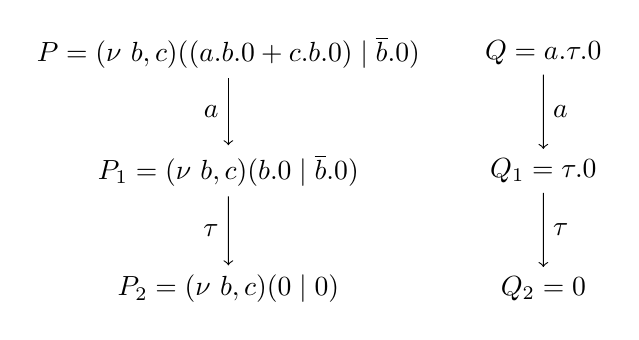
\begin{tikzpicture}
            \node at (0, 0) {$P = (\nu \ b, c)((a.b.0 + c.b.0) \mid \overline{b}.0)$}
            child {
                node {$P_1 = (\nu \ b, c)(b.0 \mid \overline{b}.0)$}
                child {
                    node {$P_2 = (\nu \ b, c)(0 \mid 0)$}
                    edge from parent[->] node[left] {$\tau$}
                }
                edge from parent[->] node[left] {$a$}
            };

            \node at (4, 0) {$Q = a.\tau.0$}
            child {
                node {$Q_1 = \tau.0$}
                child {
                    node {$Q_2 = 0$}
                    edge from parent[->] node[right] {$\tau$}
                }
                edge from parent[->] node[right] {$a$}
            };
        \end{tikzpicture}
    \end{figure}
    \noindent In this case, the relation we want is:
    \[\mathcal{R} = \{(P, Q), (P_1, Q_1), (P_2, Q_2)\}.\]
    We note that $P_2$ and $Q_2$ are strongly bisimilar since they have no transitions. Moreover, since the other processes have just one transition, with the coupled result in $\mathcal{R}$, we conclude that $\mathcal{R}$ is a strong bisimulation. Hence, $P$ and $Q$ are strongly bisimilar.

    There are many extensions to bisimulation, including:
    \begin{itemize}
        \item allowing messages, including mobile names- this requires a more complex version of the labelled transition rules; and
        \item defining \emph{weak bisimulation}, which ignores $\tau$-transitions. This allows internal interaction to be ignored and focuses on observable input-output.
    \end{itemize}
    \newpage

    \section{Types in $\pi$-calculus}
    In general, static typechecking aims to eliminate errors. In terms of $\pi$-calculus, we want to ensure that whenever a message is sent, the sender and receiver agree on its structure. In particular, we would like to eliminate processes such as:
    \begin{itemize}
        \item $\overline{a} \langle u, v \rangle.0 \mid a(x).P$, where the two subprocesses do not agree on the number of parameters; and
        \item $\overline{a} \langle \textit{true}, \textit{false} \rangle.0 \mid a(x, y).\overline{a} \langle x + y \rangle.0$, where the two subprocesses do not agree on type.
    \end{itemize}

    We will now look at \emph{simple} type system for $\pi$-calculus. It deals with these two issues by specifying:
    \begin{itemize}
        \item the number of components of messages on the channel and
        \item the type of each component.
    \end{itemize}
    We illustrate this with an example. So, assume that the channel $a$ is of type $\texttt{Chan}[\textit{int}, \textit{bool}]$, denoted by $a \colon \texttt{Chan}[\textit{int}, \textit{bool}]$. Then,
    \begin{itemize}
        \item $\overline{a} \langle 1 + 2, \textit{true} \rangle$ is well-typed;
        \item $a(x, y).P$ is well-typed if $x \colon \textit{int}$ and $y \colon \textit{bool}$ in $P$; while
        \item $\overline{a} \langle 1 \rangle$, $\overline{a} \langle true, 1, false \rangle$ and $a(x)$ are incorrect.
    \end{itemize}
    Instead, if $a \colon \texttt{Chan}[\texttt{Chan}[\textit{int}]]$, then $a(x).x(y).Q$ is well-typed if $y \colon \textit{int}$ in $Q$.

    Formally, types are specified by the following grammar:
    \begin{align*}
        T &:: = \texttt{Chan}[T, \dots, T] \\
        &\mid \textit{bool} \\
        &\mid \dots
    \end{align*}
    where the final line can be used for any types we would want the $\pi$-calculus to have, e.g. \textit{int}.

    As for $\lambda$-calculus, we modify the syntax of processes so that binding occurences are annotated with types, e.g.
    \[a(x_1 \colon T_1, \dots, x_n \colon T_n) \qquad (\nu \ x \colon T)\]
    
    We will consider \emph{polyadic $\pi$-calculus}. This means that a message has zero or more components. We will also assume that the expression language has a type system with types \textit{int} and \textit{bool}, along with appropriate reduction relations involving them.

    Now, we define the modified syntax of $\pi$-calculus, including processes $P$, values $v$ and expressions $e$:
    \begin{align*}
        P &::= 0  & \textrm{terminated process} \\
        &\mid \overline{x} \langle e_1, \dots, e_n \rangle.P & \textrm{output/send} \\
        &\mid x(y_1 \colon T_1, \dots, y_n \colon T_n).P & \textrm{input/receive} \\
        &\mid (\nu  \ x \colon T)P & \textrm{scope/restriction} \\
        &\mid P \mid Q & \textrm{parallel composition} \\
        &\mid P + Q & \textrm{choice} \\
        &\mid \dots \\
        v &::= x & \textrm{channel names} \\
        &\mid \textit{true}, \textit{false} & \textrm{boolean values} \\
        &\mid \dots \\
        e &::= v & \textrm{values} \\
        &\mid e == e & \textrm{equality expressions} \\
        &\mid \dots
    \end{align*}
    The dots ($\dots$) allow for expansion of the syntax as required.

    Assuming \emph{call-by-value}, the reduction rule for communication, with polyadic messages, is:
    \begin{align*}
        (x(y_1 \colon T_1, \dots, y_n \colon T_n).P + \dots) &\mid 
        (\overline{x}\langle v_1, \dots, v_n \rangle.Q + \dots) \\
        &\downarrow \\
        P[y_1 := v_1, \dots, y_n := v_n] &\mid Q
    \end{align*}
    If $n = 0$, then we do not send/receive any message- this is synchronisation. If we have a send and a receive on the same channel with different number of components in message, then there is no reduction. This is a \emph{communication error}. We define the type system in a way that avoids such errors.

    Let $\Gamma = x_1 \colon T_1, \dots, x_n \colon T_n$ be a \emph{typing context} or \emph{typing environment}. We have typing judgment for processes and expressions.
    \begin{itemize}
        \item The \emph{typing judgment for processes} is $\Gamma \vdash P$ (i.e. under $\Gamma$, $P$ is a well-typed process). A process does not have a type- the judgment just says that it uses channels in $\Gamma$ correctly. 
        \item The \emph{typing judgment for expressions} is $\Gamma \vdash e \colon T$ (i.e. under $\Gamma$, the expression $e$ has type $T$). This is similar to simply typed $\lambda$-calculus. It includes the case where $e$ is just a channel name.
    \end{itemize}
    
    We now define the typing rules. The process $0$ is well-typed in any environment:
    \[\frac{}{\Gamma \vdash 0} \textrm{TNil}.\]
    Well-typed processes can be put in parallel, or used as alternatives.
    \[\frac{\Gamma \vdash P \quad \Gamma \vdash Q}{\Gamma \vdash P \mid Q} \textrm{TPar} \qquad \frac{\Gamma \vdash P \quad \Gamma \vdash Q}{\Gamma \vdash P + Q} \textrm{TPlus}\]
    An output must send a message of the correct structure.
    \[\frac{\Gamma \vdash x \colon \texttt{Chan}[T_1, \dots, T_n] \quad \Gamma \vdash e_i \colon T_i \ \forall 1 \leq i \leq n \quad \Gamma \vdash P}{\Gamma \vdash \overline{x} \langle e_1, \dots, e_n\rangle.P} \textrm{TOut}\]
    In an input, the message must have the correct structure, and its components must be used correctly.
    \[\frac{\Gamma \vdash x \colon \texttt{Chan}[T_1, \dots, T_n] \qquad \Gamma, y_1 \colon T_1, \dots, y_n \colon T_n \vdash P}{\Gamma \vdash x(y_1 \colon T_1, \dots, y_n \colon T_n).P} \textrm{TIn}\]
    When a new channel is created, it must be used correctly.
    \[\frac{\Gamma, x \colon \texttt{Chan}[T_1, \dots, T_n] \vdash P}{\Gamma \vdash (\nu \ x \colon \texttt{Chan}[T_1, \dots, T_n]) P} \textrm{TNew}\]

    We now illustrate the types with an example. So, consider the following processes:
    \begin{align*}
        \textit{Server} &= a(x).x(y).\overline{x} \langle y + 1 \rangle.0 \\
        \textit{Client} &= (\nu \ c)\overline{a} \langle c \rangle.\overline{c} \langle 2 \rangle.c(z).0
    \end{align*}
    We can see that:
    \begin{itemize}
        \item $a$ has type $\texttt{Chan}[\texttt{Chan}[\textit{int}]]$;
        \item $x$ has type $\texttt{Chan}[\textit{int}]$;
        \item $c$ has type $\texttt{Chan}[\textit{int}]$;
        \item $y$ (and $y+1$) has type $\textit{int}$; and
        \item $z$ has type $\textit{int}$.
    \end{itemize}
    So, we can define $\Gamma$ to be the typing context with all these types. Then, $\Gamma \vdash \textit{Server} \mid \textit{Client}$.
    % So, let $\Gamma$ be the typing judgment with these types. We can then construct the typing derivation for the $\textit{Server}$ as follows:
    % \[\nfrac{
    %     \Gamma \vdash a \colon \textit{Chan}[\texttt{Chan}[\textit{int}]] \nfrac{
    %         \Gamma \vdash x \colon \texttt{Chan}[\textit{int}] \quad \nfrac{
    %             \Gamma \vdash x \colon \texttt{Chan}[\textit{int}] \quad \Gamma \vdash y + 1 \colon \textit{int}
    %         }{
    %             \Gamma, y \colon \textit{int} \vdash \overline{x} \langle y + 1 \rangle.0
    %         } \textrm{TOut}
    %     }{\Gamma, x \colon \texttt{Chan}[\textit{int}] \vdash x(y).\overline{x} \langle y + 1 \rangle.0} \textrm{TIn}
    % }{
    %     \Gamma \vdash a(x).x(y).\overline{x} \langle y + 1 \rangle.0
    % } \textrm{TIn}\]

    % \begin{tabular}{cccccccccc}
    %     && $\Gamma \vdash x \colon \texttt{Chan}[\textit{int}]$ & \quad & $\Gamma \vdash y + 1 \colon \textit{int}$ & \multirow{2}{*}{TOut} \\
    %     \cline{3-5} 
    %     & $\Gamma \vdash x \colon \texttt{Chan}[\textit{int}]$ & \multicolumn{3}{c}{$\Gamma, y \colon \textit{int} \vdash \overline{x} \langle y + 1 \rangle.0$} & \multirow{2}{*}{TIn}\\
    %     \cline{2-5} 
    %     $\Gamma \vdash a \colon \texttt{Chan}[\texttt{Chan}[\textit{int}]]$ &&& $\Gamma, x \colon \texttt{Chan}[\textit{int}] \vdash x(y).\overline{x} \langle y + 1 \rangle.0$ 
    % \end{tabular}

    The simple type system for $\pi$-calculus has issues. In particular, 
    \begin{itemize}
        \item deadlock procesess are typeable, e.g. $\overline{b}\langle \textit{true} \rangle.0 \mid c(y \colon \textit{int}).0$; and
        \item recursive processes are not typeable, even though they should be.
    \end{itemize}
    
    Nonetheless, we will show that the simple type system is safe. This can be done by showing:
    \begin{itemize}
        \item \emph{type preservation}: if $\Gamma \vdash P$ and $P \to Q$, then $\Gamma \vdash Q$;
        \item \emph{absence of immediate communication errors}: if $\Gamma \vdash P$ at the top level, $P$ does not have an input and an output in parallel on the same channel with different number of message components (and types).
    \end{itemize}
    Proving these theorems allows us to show that well-typed processes do not generate communication errors.

    To prove these theorems, we need some auxiliary results.
    \begin{lemma}[Substitution in Processes]
        If $\Gamma, x_1, \colon T_1, \dots, x_n \colon T_n$ and for each $1 \leq i \leq n$, $\Gamma \vdash v_i \colon T_i$, then 
        \[\Gamma \vdash P[x_1 := v_1, \dots, x_n := v_n].\]
    \end{lemma}
    \noindent If $v_i$ are only allowed to be channel names, then we can prove this by induction on the derivation of $\Gamma \vdash P$.

    Next, to handle values in the expression language, we need a similar lemma for substitution in expressions.
    \begin{lemma}[Substitution in Expressions]
        If $\Gamma, x_1 \colon T_1, \dots, x_n \colon T_n \vdash e \colon T$ and for $1 \leq i \leq n$, $\Gamma \vdash v_i \colon T_i$, then
        \[\Gamma \vdash e[x_1 := v_1, \dots, x_n := v_n] \colon T.\]
    \end{lemma}
    \noindent This can also be proved using induction.

    Because reduction allows the use of structural congruence, we need to prove that this does not affect typeability.
    \begin{lemma}
        If $\Gamma \vdash P$ and $P \equiv Q$, then $\Gamma \vdash Q$.
    \end{lemma}
    \noindent We can prove this by structural induction on $\equiv$. In particular, we consider that $P$ is typeable and then show that $Q$ is typeable, and vice versa.
    \begin{proof}[Proof for scope expansion]
        The rule for structural congruence tells us that for processes $P$ and $Q$, and a channel $x \not\in FV(P)$,
        \[(\nu \ x)(P \mid Q) \equiv P \mid (\nu \ x)Q.\]
        If the left hand side is typeable, then we have
        \[\cfrac{\Gamma, x \colon T \vdash P \quad \Gamma, x \colon T \vdash Q}{\cfrac{\Gamma, x \colon T \vdash P \mid Q}{\Gamma \vdash (\nu \ x \colon T)(P \mid Q)}}\]
        using TPar and then TNew. Hence, we need $\Gamma, x \colon T \vdash P$ and $\Gamma, x \colon T \vdash Q$ for the left hand side to be typeable. Since $x \not\in FV(P)$, we can show that $\Gamma \vdash P$. Hence,
        \[\cfrac{\Gamma, x \colon T \vdash Q}{\cfrac{\Gamma \vdash P \quad \Gamma \vdash (\nu \ x \colon T)Q}{\Gamma \vdash P \mid (\nu \ x \colon T)Q}}\]
        using TNew and then TPar. So, if the left hand side is typeable, then so is the right hand side. Using the reverse argument, we can show that if the right hand side is typeable, then so is the left hand side.
    \end{proof}

    We now prove type preservation.
    \begin{theorem}[Type Preservation]
        If $\Gamma \vdash P$ and $P \to Q$, then $\Gamma \vdash Q$.
    \end{theorem}
    We prove this using structural induction on $P \to Q$, by considering each case for the reduction step. In each case, we then analyse the structure of the derivation of $\Gamma \vdash P$ and use the component parts to show that $\Gamma \vdash Q$. The key case is that of communication, where we have
    \[x(y_1 \colon T_1, \dots, y_n \colon T_n).P \mid \overline{x} \langle v_1, \dots, v_n \rangle.Q \to P[y_1 := v_1, \dots, y_n := v_n] \mid Q.\]
    We ignore non-deterministic choice for simplicity. The typing derivation of the left hand side has the following form:
    \[
    \setstackgap{S}{4pt}
    \cfrac{
        \cfrac{\Shortstack[c]
            {
                \Gamma \vdash x \colon \texttt{Chan}[T_1, \dots, T_n] \\
                \Gamma, y_1 \colon T_1, \dots, y_n \colon T_n  \vdash P 
            }
        }{
            \Gamma \vdash x(y_1 \colon T_1, \dots, y_n \colon T_n).P
        } \textrm{TIn} \qquad \cfrac{\Shortstack[c]
            {
                \Gamma \vdash x \colon \texttt{Chan}[T_1, \dots, T_n] \\
                \Gamma \vdash v_1 \colon T_1, \dots, v_n \colon T_n \qquad \Gamma \vdash Q 
            }
        }{
            \Gamma \vdash \overline{x} \langle v_1, \dots, v_n \rangle.Q 
        } \textrm{TOut}
    }{
        \Gamma \vdash x(y_1 \colon T_1, \dots, y_n \colon T_n).P \mid \overline{x} \langle v_1, \dots, v_n \rangle.Q
    } \textrm{TPar}\]
    Using the Substitution Lemma 1 and the typing derivations, we get that
    \[\Gamma \vdash P[y_1 := v_1, \dots, y_n := v_n]\]
    Using TPar, we can derive that
    \[\Gamma \vdash P[y_1 := v_1, \dots, y_n := v_n] \mid Q,\]
    hence the right hand side is well-typed. The other cases use induction in a similar manner.

    We will now give a precise statement that \emph{a well-typed process does not have immediate communication errors}. First, we can use scope expansion to write any process in the form
    \[(\nu \ x_1) \dots (\nu \ x_n)(P_1 \mid \dots \mid P_n),\]
    where immediate communications among the $P_i$ are at the top level and not within $\nu$ operators.
    \begin{theorem}[Absence of immediate communication errors]
        If 
        \[\Gamma \vdash (\nu \ x_1 \colon T_1, \dots, x_k \colon T_k)(x(y_1 \colon U_1, \dots, y_r \colon U_r).P \mid \overline{x} \langle v_1, \dots, v_n \rangle.Q)\]
        then
        \begin{itemize}
            \item $n = r$ and
            \item $\Gamma \vdash v_i \colon U_i$ for all $1 \leq i \leq n$.
        \end{itemize}
    \end{theorem}
    \noindent So, the number of message components is the same as in the input and the output, and the messages/values components are of the types expected by the input.
    \begin{proof}
        The typing derivation must have the form
        \[\Gamma_1 = \Gamma, x_1 \colon T_1, \dots, x_n \colon T_m.\]
        % TODO: Draw the derivation
        Considering $\Gamma \vdash x(y_1 \colon U_1, \dots, y_r \colon U_r).P$, $\Gamma_1$ must contain $x \colon \texttt{Chan}[U_1, \dots, U_r]$. Moreover, since $\Gamma \vdash \overline{x} \langle v_1, \dots, v_n \rangle.Q$, we see that $x \colon \texttt{Chan}[U_1, \dots, U_r]$ in the derivation. Hence, $n = r$ and $\Gamma \vdash v_i \colon U_i$ for $1 \leq i \leq n$.
    \end{proof}

    The simple type system for $\pi$-calculus provides a way of statically checking that communication channels are used consistently throughout a program. This eliminates a certain class of communication errors.
    
    Several type systems have been developed for the $\pi$-calculus. Some aim to classify channels in more precise ways (input/output, linear, polymorphic, etc.). Others aim to eliminate more complex behavioural errors, such as deadlocks and livelocks. Lastly, behavioural type systems specify \emph{order} and \emph{sequence} of send and receive.
    
    \subsection{Advanced Types}
    We will now look at an advanced type system for $\pi$-calculus that aims to classify channels in a more precise way.

    A fairly straightforward refinement of the simple type system introduces two new channel type constructors:
    \begin{itemize}
        \item $\texttt{In}[T_1, \dots, T_n]$ is the type of channels that can be used to \emph{input} messages of type $T_1, \dots, T_n$; and
        \item $\texttt{Out}[T_1, \dots, T_n]$ is the type of channels that can be used to \emph{output} messages of type $T_1, \dots, T_n$.
    \end{itemize}
    Now, types are specified by the following grammar:
    \begin{align*}
        T &::= \texttt{Chan}[T_1, \dots, T_n] \\
        &\mid \texttt{In}[T_1, \dots, T_n] \\
        &\mid \texttt{Out}[T_1, \dots, T_n] \\
        &\mid \dots
    \end{align*}
    
    Input/output channel types introduce a notion of \emph{subtyping}. A subtyping relation connects the new constructors and the original constructor:
    \begin{align*}
        \texttt{Chan}[T_1, \dots, T_n] &<: \texttt{In}[T_1, \dots, T_n] \\
        \texttt{Chan}[T_1, \dots, T_n] &<: \texttt{Out}[T_1, \dots, T_n] 
    \end{align*}

    The following defines the subtyping rules in general- we have reflexivity and transitivity, which make it a partial order:
    \[\frac{}{T <: T} \textrm{SRefl} \qquad \frac{R <: S \qquad S <: T}{R <: T} \textrm{STrans}\]
    We also have the rules we saw above:
    \[\frac{}{\texttt{Chan}[T_1, \dots, T_n] <: \texttt{In}[T_1, \dots, T_n]} \textrm{SChanIn}\]
    \[\frac{}{\texttt{Chan}[T_1, \dots, T_n] <: \texttt{Out}[T_1, \dots, T_n]} \textrm{SChanOut}\]
    We have covariance in subtyping with respect to input:
    \[\frac{S_1 <: T_1 \qquad \dots \qquad S_n <: T_n}{\texttt{In}[S_1, \dots, S_n] <: \texttt{In}[T_1, \dots, T_n]} \textrm{SInIn}\]
    In terms of programming, consider the types \textit{num} and its subtype \textit{num}. Then, a channel accepting \textrm{num} can accept a value of type \textit{int}. We have contravariance in subtyping with respect to output:
    \[\frac{T_1 <: S_1 \qquad \dots \qquad T_n <: S_n}{\texttt{Out}[S_1, \dots, S_n] <: \texttt{Out}[T_1, \dots, T_n]} \textrm{SOutSOut}\]
    In terms of programming, a channel that outputs an \textit{int} can be thought of as a channel that outputs \textit{num}. For subtyping with a general channel, we require both covariance and contravariance:
    \[\frac{S_1 <: T_1 \qquad \dots \qquad S_n <: T_n \qquad T_1 <: S_1 \qquad \dots \qquad T_n <: S_n}{\texttt{Chan}[S_1, \dots, S_n] <: \texttt{In}[T_1, \dots, T_n]} \textrm{SChanChan}\]
    To make use of subtyping, the typing judgment can be extended with the subsumption rule:
    \[\frac{\Gamma \vdash x \colon S \qquad S <: T}{\Gamma \vdash T} \textrm{TSub}\]

    An output must send a message of the correct structure on a channel having an output channel type. The inference rule is now:
    \[\frac{\Gamma \vdash x \colon {\color{red}\texttt{Out}[T_1, \dots, T_n]} \quad \Gamma \vdash e_i \colon T_i \ \forall 1 \leq i \leq n \quad \Gamma \vdash P}{\Gamma \vdash \overline{x} \langle e_1, \dots, e_n \rangle.P} \textrm{TOut}\]
    The change is highlighted in red- we have \texttt{Out} instead of \texttt{Chan}. 

    In an input, the message must have the correct structure and its components must be used correctly.
    \[\frac{\Gamma \vdash x \colon {\color{red}\texttt{In}[T_1, \dots, T_n]} \qquad \Gamma, y_1 \colon T_1, \dots, y_n \colon T_n \vdash P}{\Gamma \vdash x(y_1 \colon T_1, \dots, y_n \colon T_n).P} \textrm{TIn}\]
    A channel can only be created of type \texttt{Chan} in TNew; it cannot be the other way round.

    % TODO: The exercises

    In addition to capabilities of input/output, channel types can be refined by introducing \emph{multiplicities} for linear and shared channels. \emph{Linearity} restricts channel usage exactly once, in accordance with its capability:
    \begin{itemize}
        \item linear input type $\ell_i[\cdot]$ can only be used once in input;
        \item linear output type $\ell_o[\cdot]$ can only be used once in output; and
        \item linear channel type $\ell_{\textit{Chan}}[\cdot]$ can only be used once in input and output.
    \end{itemize}
    Linear types allow for resource-aware programming and have inspired ownership types and unique types in PLs. The updated types are the following:
    \begin{align*}
        T &::= \texttt{Chan}[T_1, \dots, T_n] \\
        &\mid \ell_i[T_1, \dots, T_n] \\
        &\mid \ell_o[T_1, \dots, T_n] \\
        &\mid \ell_{\textit{Chan}}[T_1, \dots, T_n] \\
        &\mid \dots
    \end{align*}

    In order to respect linearity, a linear type system must keep track of the resources used, without duplicating or discarding any. We need a notion of \emph{type combination} on types, contexts and ultimately on typing rules. We will use the symbol $\uplus$ for the type combination operator, or simply $+$.

    The combination `$\uplus$' of types is a symmetric operation and is defined by the following rules:
    \begin{align*}
        \ell_i[T_1, \dots, T_n] \uplus \ell_o[T_1, \dots, T_n] &\triangleq \ell_{\textit{Chan}}[T_1, \dots, T_n] \\
        \texttt{Chan}[T_1, \dots, T_n] \uplus \texttt{Chan}[T_1, \dots, T_n] &\triangleq \texttt{Chan}[T_1, \dots, T_n] \\
        \textit{bool} \uplus \textit{bool} &\triangleq \textit{bool} \\
        T \uplus T' &\triangleq \texttt{undef} & \textrm{otherwise}.
    \end{align*}
    Now, we extend `$\uplus$' on typing contexts based on these rules:
    \[(\Gamma_1 \uplus \Gamma_2)(x) \triangleq \begin{cases}
        \Gamma_1(x) \uplus \Gamma_2(x) & \textrm{if both } \Gamma_1(x) \textrm{ and } \Gamma_2(x) \textrm{ are defined} \\
        \Gamma_1(x) & \textrm{if } \Gamma_1(x) \textrm{ is defined but } \Gamma_2(x) \textrm{ is not defined} \\
        \Gamma_2(x) & \textrm{if } \Gamma_2(x) \textrm{ is defined but } \Gamma_1(x) \textrm{ is not defined} \\
        \texttt{undef} & \textrm{otherwise}.
    \end{cases}\]
    
    We also add typing rules for linear output and input.
    \[\frac{\Gamma_0 \vdash x \colon {\color{red}\ell_o[T_1, \dots, T_n]} \qquad \Gamma_1 \vdash e_1 \colon T_1 \quad \dots \quad \Gamma_n \colon  e_n \colon T_n \qquad \Gamma_m \vdash P}{\Gamma_0 \uplus \Gamma_i \uplus \Gamma_m \vdash \overline{x} \langle e_1, \dots, e_n \rangle.P} \textrm{TOut}\]
    \[\frac{\Gamma_0 \vdash x \colon {\color{red}\ell_i[T_1, \dots, T_n]} \qquad \Gamma_1, y_1 \colon T_1, \dots, y_n \colon T_n \vdash P}{\Gamma_0 \uplus \Gamma_1 \vdash x(y_1 \colon T_1, \dots, y_n \colon T_n).P} \textrm{TIn}\]
    Also, when a new channel is created, this must be a linear channel.
    \[\frac{\Gamma, x \colon {\color{red} \ell_{\textit{Chan}}[T_1, \dots, T_n]} \vdash P}{\Gamma \vdash (\nu \ x) \colon \ell_{\textit{Chan}}[T_1, \dots, T_n] P} \textrm{TNew}\]

    Linear type systems guarantee that resources will be used exactly once. However, a process can be built in such a way that resources are not used at all! For instance, consider the following linear process:
    \[a \colon \ell_i[\textit{bool}] \vdash (\nu \ b\colon \texttt{Chan}[\textit{bool}] )\overline{b} \langle \textit{false} \rangle.a(x).0\]
    Although this is a well-typed process under the linear type system, it is deadlocked. Further extension to types and type systems for $\pi$-calculus deal with this, along with lock freedom and termination.
    \newpage

    \section{Session Types}
    In complex distributed systems, communicating participants agree on a protocol to follow, specifying \emph{type} and \emph{direction} of data exchanged. \emph{Session types} are a type formalism used to model structured communication-based programming. They guarantee \emph{privacy}, \emph{communication safety} and \emph{session fidelity}. It was initially designed for $\pi$-calculus, but has now been designed for functional languages, object-oriented languages, and more!

    Session types were introduced in the early 90s. Since their appearance, they have developed into a significant theme in programming languages. This is because computing has now moved from the era of data processing to the era of communication. \emph{Data types} codify the structure of \emph{data} and make it available to programming tools. Similarly, \emph{session types} codify the structure of \emph{communication} and make it available to programming tools.

    We will now have a look at an example of session types using a server and a client. The session type for the server is given as follows:
    \begin{align*}
        S \triangleq \&  \{ &\textit{add} \colon ?\textit{int}. ?\textit{int}. !\textit{int}. S \\
        & \textit{neg} \colon ?\textit{int}. !\textit{int}. S \\
        & \textit{quit} \colon \textit{end} \}
    \end{align*}
    The symbol $\&$ denotes that the server $S$ is offering 3 services- \textit{add}, \textit{neg} and \textit{quit}. This is called \emph{external choice} (i.e. the client chooses). The \textit{quit} service would end in termination of the protocol. On the other hand, the \textit{add} service takes in 2 integers (as denoted by $?\textit{int}$) and then returns an integer (as denoted by $!\textit{int}$). Similarly, \textit{neg} takes an integer and returns an integer.

    From the client endpoint, the session type is the following:
    \begin{align*}
        C \triangleq \oplus \{ &\textit{add} \colon !\textit{int}. !\textit{int}. ?\textit{int}. C \\
        & \textit{neg} \colon !\textit{int}. ?\textit{int}. C \\
        & \textit{quit} \colon \textit{end} \}
    \end{align*}
    The symbol $\oplus$ denotes that the client must select one of the 3 services. This is called \emph{internal choice}. Note that a send in the server is a receive in the client and vice versa. This is called \emph{duality}, and is denoted $S = \overline{C}$.

    We will now instantiate a server $srv$. It is parametrised on the channel endpoint:
    \begin{align*}
        srv(x \colon S) = x \vartriangleright \{ &\textit{add} \colon x(a \colon \textit{int}). x(b \colon\textit{int}). \overline{x} \langle a + b \rangle. srv(x) \\
        & \textit{neg} \colon x(a \colon \textit{int}). \overline{x}\langle -a \rangle. srv(x) \\
        & \textit{quit} \colon 0 \}
    \end{align*}
    Next, we instantiate a client $clt$. It is of type $C$:
    \[clt(x \colon C) = x \vartriangleleft \textit{neg}.\overline{x} \langle 2 \rangle.x(a \colon \textit{int}).x \vartriangleleft \textit{quit}.P(a)\]
    Note that since $\oplus$ denotes an internal choice, the client $clt$ has already chosen a sequence- it first chooses the \textit{neg} service and then \textit{quit}.

    We can put $srv$ and $clt$ in parallel for communication to occur, using the reduction rules:
    \begin{align*}
        (\nu \ c \colon S)(srv(c^+) &\mid clt(c^-)) \\
        &\downarrow \\
        (\nu \ c \colon ?\textit{int}.!\textit{int}.S)(c^+(a \colon \textit{int}).\overline{c^+}\langle -a \rangle.srv(c^+) &\mid \overline{c^-}\langle 2 \rangle. c^-(a \colon \textit{int}).c^{-} \vartriangleleft \textit{quit}.P(a)) \\
        &\downarrow \\
        (\nu \ c \colon !\textit{int}.S)(\overline{c^+}\langle -2 \rangle.srv(c^+) &\mid c^-(a \colon \textit{int}). c^- \vartriangleleft \textit{quit}.P(a)) \\
        &\downarrow \\
        (\nu \ c \colon S)(srv(c^+) &\mid c^- \vartriangleleft \textit{quit}.P(-2)) \\
        &\downarrow \\
        (\nu \ c \colon \textit{end})(0 &\mid P(-2)) \\
        &\equiv \\
        & P(-2)
    \end{align*}
    The communication occurs at channel $c$. The server and the client are at the opposite ends of the channel. To distinguish this, we make use of polarities- $c^+$ for one and $c^-$ for the other. We keep track of the type using the server; the client type could have also been used here. Note that the type of the channel $c$ is given as the type of the server, and changes during the reduction process.

    As we can see, the communication occurs in a private channel $c$. To accommodate this, the server listens on a standard channel $a$ of type $\texttt{Chan}[S]$ and receives a session channel for $srv$ to use. That is,
    \[\textit{server}(a) = a(x \colon S).srv(x)\]
    The global declaration $a \colon \texttt{Chan}[S]$ advertises the server and its protocol. The client creates a session channel and sends it to the server, i.e.
    \[\textit{client}(a) = (\nu \ c \colon S)(\overline{a}\langle c^+ \rangle.clt(c^-))\]
    After one step reduction of $\textit{server}(a) \mid \textit{client}(a)$, execution proceeds as above.

    The main features of session types are the following:
    \begin{itemize}
        \item \emph{Duality}- the relationship between types of opposite endpoints of a session channel;
        \item \emph{Linearity}- each channel endpoint occurs exactly once in a collection of parallel processes;
        \item The \emph{structure} of session types matches the structure of communication;
        \item Session types \emph{change} as communication occurs;
        \item \emph{Connection} is established among participants before communication begins.
    \end{itemize}
    Session types guarantee the following:
    \begin{itemize}
        \item \emph{communication safety}- the exchanged data has the expected type;
        \item \emph{session fidelity}- the session channel has the expected structure; and
        \item \emph{privacy}- the session channel is owned only by the communicating parties.
    \end{itemize}
    This allows us to conclude that, at runtime, communication follows the protocol.

    We will now define session types using a grammar:
    \begin{align*}
        S &::= \textit{end} & \textrm{termination} \\
        & !T.S & \textrm{send} \\
        &?T.S & \textrm{receive} \\
        &\oplus \{I_i \colon S_i\}_{i \in I} & \textrm{select} \\
        &\& \{I_i \colon S_i\}_{i \in I} & \textrm{branch} 
    \end{align*}
    The value $T$ refers to a type. Now, session types are also types in $\pi$-calculus. The syntax of the processes has also changed, to the following grammar:
    \begin{align*}
        P, Q &::= 0 & \textrm{inaction} \\
        & P \mid Q & \textrm{composition} \\
        & (\nu \ x)P & \textrm{restriction} \\
        & \overline{x^p} \langle v^q \rangle.P & \textrm{output} \\
        & x^p (y).P & \textrm{input} \\
        & x^p \vartriangleleft l_j.P & \textrm{selection} \\
        & x^p \vartriangleright \{I_i \colon P_i\}_{i \in I} & \textrm{branching}
    \end{align*}
    The value $v$ refers to values, which includes channel names and other values (e.g. booleans). The values $p$ and $q$ are optional polarities for channels (i.e. $+$ or $-$).

    The typing rules are given as follows:
    \begin{align*}
        \frac{\Gamma_1 \vdash P \quad \Gamma_2 \vdash Q}{\Gamma_1 + \Gamma_2 \vdash P \mid Q} & \textrm{TPar} \\
        \frac{\Gamma, x^p \colon S, x^{\overline{p}} \colon \overline{S} \vdash P}{\Gamma \vdash (\nu \ x)P} & \textrm{TRes} \\
        \frac{\Gamma, x^p \colon S, y \colon T \vdash P}{\Gamma, x^p \colon ?T.S \vdash x^p(y).P} &\textrm{TIn} \\
        \frac{\Gamma_1, x^p \colon S \vdash P \quad \Gamma_2 \vdash v^q \colon T}{(\Gamma_1, x^p \colon !T.S) + \Gamma_2 \vdash \overline{x^p} \langle v^q \rangle.P} &\textrm{TOut} \\
        \frac{\Gamma, x^p \colon S_i \vdash P_i}{\Gamma, x^p \colon \& \{I_i \colon S_i\}_{i \in I} \vdash x^p \vartriangleright \{I_i \colon P_i\}_{i \in I}} & \textrm{TBrch} \\
        \frac{j \in I \quad \Gamma, x^p \colon S_j \vdash P}{\Gamma, x^p \colon \oplus \{I_i \colon S_i\}_{i \in I} \vdash x^p \vartriangleleft I_j.P} & \textrm{TSel}
    \end{align*}
    For a polarity $p$, its dual is denoted by $\overline{p}$. Note that the types change as we saw above.

    We define the combination $+$ operation on typing judgments as follows:
    \begin{align*}
        \Gamma + x^+ \colon S &= \Gamma, x^+ \colon S & \textrm{if } x, x^+ \not\in \operatorname{dom}(\Gamma) \\
        \Gamma + x^- \colon S &= \Gamma, x^- \colon S & \textrm{if } x, x^- \not\in \operatorname{dom}(\Gamma) \\
        \Gamma + x \colon S &= \Gamma, x \colon S & \textrm{if } x, x^+, x^- \not\in \operatorname{dom}(\Gamma) \\
        (\Gamma, x \colon T) + x \colon T &= \Gamma, x \colon T & \textrm{if } T \textrm{ is not a session type}
    \end{align*}

    We will now have a look at some terms and see whether they are well-typed:
    \begin{itemize}
        \item The process
        \[(\nu \ x)(x^+(t \colon \textit{bool}).0 \mid \overline{x^-} \langle \textit{true} \rangle.0)\]
        is well-typed since the types of $x^+$ and $x^-$ are dual.

        \item The process
        \[(\nu \ x)(\overline{x^+} \langle t \rangle.0 \mid \overline{x^-}\langle \textit{true} \rangle.0)\]
        is not well-typed since both $x^+$ and $x^-$ send data, and hence are not dual of each other.
        
        \item The process
        \[(\nu \ x)(\overline{x^-} \langle \textit{false} \rangle.0 \mid x^+ (t \colon \textit{bool}).0 \mid x^+(w \colon \textit{bool}).0)\]
        is not well-typed since it violates linearity- there can only be one occurrence of $x^+$ and $x^-$.

        \item The process
        \[(\nu x)(\nu y)(x^+(z \colon \textit{int}).\overline{y^-}\langle 42 \rangle.0 \mid \overline{x^-} \langle 11 \rangle.y^+(w \colon \textit{int}).0)\]
        is well-typed since the types of $x^-, x^+$ and $y^-, y^+$ are dual.

        \item The process
        \[(\nu x)(\nu y)(\overline{y^-}\langle 42 \rangle.x^+(z \colon \textit{int}).0 \mid \overline{x^-} \langle 11 \rangle.y^+(w \colon \textit{int}).0)\]
        is well-typed since the types of $x^-, x^+$ and $y^-, y^+$ are dual, even though the process is actually deadlocked.

        \item The process
        \[(\nu \ x)(x^- \vartriangleleft k.0 \mid x^+ \vartriangleright \{l_i \colon P_i\}_{i \in I}.0)\]
        is well-typed if and only if $k = l_i$ for some $i \in I$.
    \end{itemize}

    \subsection{Standard types and session types}
    We will now aim to connect standard types (e.g. the simple type system $\pi$-calculus) on $\pi$-calculus and session types. We saw the following types:
    \begin{itemize}
        \item $\texttt{Chan}[T_1, \dots, T_n]$ for input/output for data of type $T_1, \dots, T_n$;
        \item $\texttt{In}[T_1, \dots, T_n]$ and $\texttt{Out}[T_1, \dots, T_n]$ for only input or only output for data of type $T_1, \dots, T_n$;
        \item $\ell_i[T_1, \dots, T_n]$ and $[\ell_o[T_1, \dots, T_n]]$ for only linear input or linear output (i.e. transmit data exactly once); and
        \item \emph{variant types} $\langle l_1 \colon T_n, \dots, l_n \colon T_n \rangle$ for a disjoint union of types that are labelled.
    \end{itemize}
    On the other hand, session types have:
    \begin{enumerate}
        \item structure;
        \item duality;
        \item restriction; and
        \item branch/select.
    \end{enumerate}
    This can also be seen in standard $\pi$-calculus. In particular,
    \begin{enumerate}
        \item \emph{linearity} forces a channel to be used exactly once;
        \item we have the \emph{capability} to split a channel into input/output channels;
        \item we have \emph{restriction} that allows for creation of private channels; and
        \item \emph{variant type} allows for choice.
    \end{enumerate}
    Because of the similarities, we might ask about the difference in expressivity of standard $\pi$-calculus and session types. It turns out that they have equal expressivity.

    We can make use of standard $\pi$-calculus within session types. Hence, to prove that they have equal expressivity, we just need to show that we can convert a process that makes use of session types to a process without the session types, but the same functionality. 
    
    The encoding is based on:
    \begin{itemize}
        \item \emph{linearity} of channel types;
        \item \emph{input} and \emph{output} channel capabilities;
        \item the \emph{continuation-passing} principle; and
        \item \emph{variant types}.
    \end{itemize}
    The way the encoding works, informally, is as follows:
    \begin{itemize}
        \item session types are encoded as linear channels;
        \item $?$ and $!$ are encoded as $\ell_i$ and $\ell_o$ respectively;
        \item $\& \{I_i \mid S_i\}_{i \in I}$ and $\oplus \{I_i \mid S_i\}_{i \in I}$ are encoded using variant types;
        \item continuation of a session type becomes the carried type; and
        \item dual operations in continuation become equal when carried.
    \end{itemize}
    
    We will now consider the encoding process with an example. So, assume that $S$ is a process with session type:
    \[S = ?\textit{int}.?\textit{int}.!\textit{bool}.\textit{end}\]
    Then, it is encoded as the following type in standard $\pi$-calculus:
    \[\lVert S \rVert = \ell_i[\textit{int}, \ell_i[\textit{int}, \ell_o [\textit{bool}, \varnothing]]]\]
    As we can see, an input type $?\textit{int}$ becomes $\ell_i[\textit{int}, \cdot]$, where $\cdot$ contains the continuation process. Similarly, an output type $!\textit{int}$ becomes $\ell_o[\textit{int}, \cdot]$. Finally, \textit{end} is denoted by the empty symbol $\varnothing$.

    Now, consider the dual type of $S$:
    \[\overline{S} = !\textit{int}.!\textit{int}.?\textit{bool}.\textit{end}\]
    Then, it is encoded as the following type:
    \[\lVert \overline{S} \rVert = \ell_o[\textit{int}, \ell_i[\textit{int}, \ell_o[\textit{bool}, \varnothing]]]\]
    Note that although the first $?\textit{int}$ has been converted into $\ell_o[\textit{int}, \cdot]$, this is not the case for the second one. This is because both $S$ and its dual $\overline{S}$ have to agree on the type of input/output for them to be able to communicate. Hence, the second parameter of the dual $\overline{S}$ must be the same as the second parameter of $S$. We can also think of this as encoding its dual after a receive type. We can think of this in general- in session types, dual types have opposite types throughout, whereas in normal $\pi$-calculus, only the topmost type is of opposite type.

    Formally, the algorithm for encoding is given as follows:
    \begin{align*}
        \lVert \textit{end} \rVert &\triangleq \varnothing[] \\
        \lVert ?T.S \rVert &\triangleq \ell_i[\lVert T \rVert, \lVert S\rVert] \\
        \lVert !T.S \rVert &\triangleq \ell_o[\lVert T\rVert, \lVert\overline{S}\rVert] \\
        \lVert \& \{I_i \mid S_i\}_{i \in I} \rVert &\triangleq \ell_i[\langle l_i \mid \lVert S_i \rVert \rangle_{i \in I}] \\
        \lVert \oplus \{I_i \mid S_i\}_{i \in I} \rVert &\triangleq \ell_o[\langle l_i \mid \lVert \overline{S_i}\rVert \rangle_{i \in I}]
    \end{align*}
    
    The encoding obeys many properties, such as:
    \begin{itemize}
        \item it preserves \emph{typeability} of programs;
        \item it preserves \emph{evaluation} of programs; and
        \item encoding of dual session types gives \emph{dual linear $\pi$-types}.
    \end{itemize}

    The encoding has quite powerful applications, including:
    \begin{itemize}
        \item large usability of standard typed $\pi$-calculus theory;
        \item derivation of processes for session $\pi$-calculus from the standard $\pi$-calculus (e.g. type safety);
        \item elimination of redundancy in the syntax of types and terms, and in theory;
        \item the robustness of the encoding (subtyping, polymorphism and higher-order);
        \item expressivity result for session types;
        \item implementation of session types in mainstream programming languages.
    \end{itemize}

    \subsection{Curry-Howard Isomorphism}
    We will now look at the Curry-Howard isomorphism for session types. Since the beginning of linear logic, there were suggestions that it should be relevant to concurrency. The logically approach for session types has been studied since the 1990s. It has been extended to dependent types, failures, sharing and races.

    The correspondence between session types as linear logic is the following:
    \begin{itemize}
        \item propositions are equivalent to session types;
        \item proofs are equivalent to $\pi$-procesess; and
        \item proof normalisation and cut elimination are equivalent to communication.
    \end{itemize}
    Moreover,
    \begin{itemize}
        \item the proposition $A \parr B$ is interpreted as `input $A$ then behave like $B$', i.e. $?A.B$;
        \item the proposition $A \otimes B$ is interpreted as `output $A$ then behave like $B$', i.e. $!A.B$;
        \item $\&$ and $\oplus$ are interpreted to branch and select.
    \end{itemize}
    The correspondence has lead to a re-examination of all aspects of session types from a logical viewpoint.

    These are the connections between session types and classical linear logic.
    \begin{align*}
        \frac{{\color{red} P} \dashv \vartriangle {\color{red} y} \colon A, {\color{red} x} \colon B}{{\color{red}x(y).P} \dashv \vartriangle, x \colon A \parr B} & \textrm{T}\parr \\
        \frac{{\color{red} P} \dashv \vartriangle, {\color{red} y} \colon A \quad {\color{red} Q} \dashv \vartriangle', {\color{red} x} \colon B}{{\color{red} \overline{x} \langle y \rangle.(P \mid Q)} \dashv \vartriangle, \vartriangle', {\color{red} x} \colon A \otimes B} & \textrm{T}\otimes \\
        \frac{{\color{red} P} \dashv \vartriangle, x \colon \overline{A} \quad {\color{red} Q} \dashv \vartriangle', {\color{red} x} \colon A}{{\color{red} (\nu \ x)(P \mid Q)} \dashv \vartriangle, \vartriangle'} & \textrm{TCut} \\
        \frac{{\color{red} P_i} \dashv \vartriangle, {\color{red} x} \colon A_i}{{\color{red} x \vartriangleright \{l_i \colon P_i\}_{i \in I}} \dashv \vartriangle, {\color{red} x} \colon \&\{I_i \colon A_i\}_{i \in I}} & \textrm{T} \& \\
        \frac{{\color{red} P} \dashv \vartriangle, {\color{red} x} \colon A_j \quad j \in I}{{\color{red} x \vartriangleleft l_j.P} \dashv \Delta, {\color{red} x} \colon \oplus \{I_i \mid A_i\}_{i \in I}} & \textrm{T}\oplus 
    \end{align*}
    % TODO: Reverse judgment and type
    The red values are propositions, while the black ones are classical linear logic. Note that the judgment is reversed.

    The session type system based on classical linear logic propositions guarantees:
    \begin{itemize}
        \item type preservation (or subject reduction)- well-typed processes reduce to well-typed processes;
        \item deadlock-freedom (by design)- if a process $P$ is well-typed and it is a \emph{cut}, then there is some $Q$ such that $P$ reduces to $Q$ and $Q$ is not a \emph{cut}.
    \end{itemize}

    Curry-Howard correspondences between session-typed languages and linear logic are a vivid research area. Recent work includes extending these correspondences to include more expressive processes-containing `good' cycles, sharing, recursion, dependent types and so on.

\end{document}